% !TEX program = xelatex
%==============================================================================
%  TÀI LIỆU BÁO CÁO NGHIÊN CỨU & KỸ THUẬT
%  DỰ ÁN: LAZADA UPLIFT MODELING — CATE ESTIMATION BENCHMARK & PIPELINE
%  Tác giả: Hà Trung Kiên (Data Science & Causal ML)
%  Biên dịch: XeLaTeX
%==============================================================================
\documentclass[11pt,a4paper]{article}

%---------------- 1. Font & Ngôn ngữ (XeLaTeX) ----------------
\usepackage{fontspec}
\usepackage{polyglossia}
\setdefaultlanguage{vietnamese}
\setotherlanguage{english}

\setmainfont{TeX Gyre Termes}
\setsansfont{TeX Gyre Heros}
\setmonofont[Scale=0.86]{TeX Gyre Cursor}

%---------------- 2. Định dạng trang & Màu sắc ----------------
\usepackage[a4paper,top=2.2cm,bottom=2.2cm,left=2.2cm,right=2.2cm]{geometry}
\usepackage{setspace}
\setstretch{1.15}
\usepackage{xcolor}

\definecolor{primary}{HTML}{0288D1}      % Xanh dương Data Science
\definecolor{secondary}{HTML}{F57C00}    % Cam Data Engineering
\definecolor{darkblue}{HTML}{0D47A1}
\definecolor{darkgreen}{HTML}{2E7D32}
\definecolor{darkred}{HTML}{C62828}
\definecolor{codebg}{HTML}{F4F6F9}

%---------------- 3. Toán học & Ký hiệu Causal ----------------
\usepackage{amsmath,amssymb,amsthm,bm}
\newcommand{\Exp}{\mathbb{E}}
\newcommand{\Prob}{\mathbb{P}}
\newcommand{\indep}{\perp\!\!\!\perp}
\DeclareRobustCommand{\code}[1]{{\small\texttt{#1}}}
\newcommand{\pp}{\ensuremath{\,\text{pp}}}

%---------------- 4. Bảng biểu & Khung hiển thị ----------------
\usepackage{booktabs,tabularx,array,multirow,longtable}
\usepackage[most]{tcolorbox}
\usepackage{enumitem}
\setlist{nosep,leftmargin=1.5em}
\usepackage{graphicx}
\graphicspath{{figures/}{Latex/figures/}}
\usepackage{float}
\usepackage{caption}
\usepackage{subcaption}

%---------------- 5. TikZ (Vẽ Sơ đồ Luồng & Kiến trúc) ----------------
\usepackage{tikz}
\usetikzlibrary{shapes.geometric, arrows.meta, positioning, calc, shadows}

%---------------- 6. Trích dẫn & Hyperlink ----------------
\usepackage[colorlinks=true,linkcolor=primary,citecolor=primary,urlcolor=primary]{hyperref}
\pdfstringdefDisableCommands{%
    \def\code#1{#1}%
}

%---------------- 7. Cấu hình tcolorbox ----------------
\tcbset{
    enhanced,
    fonttitle=\bfseries\color{white},
    coltitle=white,
    boxrule=0.8pt,
    arc=4pt,
    drop shadow=black!10!white
}

\newtcolorbox{quadrantbox}[2]{
    colback=#1!5!white,
    colframe=#1!80!black,
    title=#2,
    halign=left
}

\newtcolorbox{summarybox}[1][Tóm tắt cốt lõi]{
    colback=primary!5!white,
    colframe=primary,
    title=#1
}

%==============================================================================
\begin{document}

%--- TRANG BÌA & TIÊU ĐỀ ---
\begin{titlepage}
    \centering
    \vspace*{1cm}
    {\Large \bfseries BÁO CÁO NGHIÊN CỨU THỰC NGHIỆM VÀ KỸ THUẬT}\\[1.5cm]

    \rule{\textwidth}{1.5pt}\\[0.4cm]
    {\huge \bfseries NGHIÊN CỨU CÁC PHƯƠNG PHÁP ƯỚC LƯỢNG DOUBLY ROBUST CATE CHO BÀI TOÁN UPLIFT MODELING}\\[0.3cm]
    {\large \itshape So sánh DR-Learner và Double Machine Learning (DML) định hướng nâng cấp pipeline cá nhân hóa khuyến mãi trên dữ liệu Lazada}\\[0.2cm]
    \rule{\textwidth}{1.5pt}\\[2cm]

    \begin{minipage}{0.45\textwidth}
        \begin{flushleft} \large
            \textbf{Người thực hiện:}\\
            Hà Trung Kiên\\
            Lĩnh vực: \textit{Data Science \& Causal ML}
        \end{flushleft}
    \end{minipage}
    \begin{minipage}{0.45\textwidth}
        \begin{flushright} \large
            \textbf{Thông tin dự án:}\\
            Dự án: \code{final-lazada}
        \end{flushright}
    \end{minipage}

    \vfill
    {\large \textbf{Tháng 8 năm 2026}}
\end{titlepage}

\newpage
\tableofcontents
\newpage
\listoffigures
\newpage
\listoftables
\newpage

%--- TÓM TẮT THỰC THI ---
\section*{Tóm tắt thực thi (Executive Summary)}
\addcontentsline{toc}{section}{Tóm tắt thực thi (Executive Summary)}

Báo cáo này trình bày nghiên cứu thực nghiệm về các phương pháp ước lượng
\textbf{Conditional Average Treatment Effect (CATE)} có đặc tính
\textbf{doubly robust} cho bài toán cá nhân hóa khuyến mãi (uplift modeling)
trên dữ liệu Lazada, gồm $926\,669$ quan sát và $181\,669$ mẫu từ thử nghiệm
ngẫu nhiên có đối chứng (RCT). Nghiên cứu so sánh DR-Learner
\cite{kennedy2020}, các biến thể Double Machine Learning (LinearDML,
NonParamDML và CausalForestDML) \cite{chernozhukov2018}, cùng hai mô hình cơ
sở S-Learner và T-Learner.

\textbf{Các kết quả và đóng góp chính:}
\begin{enumerate}
    \item \textbf{Thiết kế thực nghiệm:} Chia dữ liệu cố định thành
    \code{Train} (80\% observational), \code{Val} (20\% observational),
    \code{RCT-select} (50\% RCT) và \code{RCT-holdout} (50\% RCT). Tập
    \code{RCT-holdout} chỉ được dùng ở bước đánh giá cuối.
    \item \textbf{Lựa chọn mô hình:} DRLearner được chọn trên
    \code{RCT-select} theo Qini Score và vượt có ý nghĩa thống kê 2 trong 5
    đối thủ. Trên \code{RCT-holdout}, mô hình đạt Qini $0.0232$ với khoảng
    tin cậy bootstrap 95\% $[-0.0007,\,0.0483]$. Khoảng này chứa 0 nên chưa
    đủ bằng chứng để khẳng định khả năng xếp hạng tốt hơn ngẫu nhiên ở mức
    ý nghĩa 5\%.
    \item \textbf{Ablation và feature contract:} Trong 76 đầu vào mô hình,
    62 đặc trưng sống tái tạo đúng dự đoán của mô hình trên phép kiểm chứng
    đã thực hiện. Handoff DS xác định 59 cột nguồn để cung cấp 55 cột trực
    tiếp và tính đầy đủ 7 đặc trưng dẫn xuất; runtime DE hiện sync 55 cột và
    giữ bốn dependency còn lại ở default, được phân tích ở phần triển khai.
    \item \textbf{Đóng gói và serving:} Ba artifact
    \code{model\_booster.txt}, \code{feature\_contract.json} và
    \code{metadata.json} được bàn giao nguyên byte sang repo hạ tầng. FastAPI
    nạp model bất biến từ Docker image, đọc feature từ Redis, cung cấp suy
    luận đơn lẻ và theo lô, đồng thời công khai health, readiness và metrics.
\end{enumerate}

\section{Giới thiệu và đặt vấn đề nghiên cứu}

\subsection{Bài toán cá nhân hóa khuyến mãi tại Lazada}
Trong các nền tảng thương mại điện tử lớn như Lazada, ngân sách dành cho các chương trình khuyến mãi (voucher giảm giá, freeship) chiếm một tỷ trọng rất lớn trong chi phí vận hành. Phương pháp phát voucher đại trà hoặc phát dựa trên các quy tắc thủ công (heuristics) thường dẫn đến việc lãng phí ngân sách nghiêm trọng do tặng nhầm đối tượng.

Khung uplift marketing thường mô tả khách hàng bằng \textbf{bốn nhóm phản
ứng tiềm ẩn} dựa trên hai kết quả đối chứng khi có và không có voucher. Đây
là cách diễn giải ở cấp độ potential outcomes; từ dữ liệu quan sát, ta không
thể biết đồng thời cả hai kết quả của cùng một cá nhân.

\vspace{0.5em}
\begin{figure}[H]
\centering
\begin{tabularx}{\textwidth}{XX}
\begin{quadrantbox}{gray}{1. Sure Things (Nhóm tự nhiên chuyển đổi)}
\begin{itemize}
    \item \textbf{Hành vi:} Không tặng voucher $\rightarrow$ Vẫn mua hàng.
    \item \textbf{Tác động:} \textcolor{darkred}{\textbf{Tốn tiền thừa!}} Phát voucher làm giảm biên lợi nhuận mà không tăng doanh số.
\end{itemize}
\end{quadrantbox}
&
\begin{quadrantbox}{gray}{2. Lost Causes (Nhóm không phản hồi)}
\begin{itemize}
    \item \textbf{Hành vi:} Tặng voucher $\rightarrow$ Vẫn không mua hàng.
    \item \textbf{Tác động:} Hoạt động tiếp cận không tạo thêm chuyển đổi và có thể phát sinh chi phí vận hành.
\end{itemize}
\end{quadrantbox}
\\
\begin{quadrantbox}{darkred}{3. Sleeping Dogs (Nhóm phản ứng ngược)}
\begin{itemize}
    \item \textbf{Hành vi:} Không tặng $\rightarrow$ Mua; tặng voucher $\rightarrow$ Không mua.
    \item \textbf{Tác động:} \textcolor{darkred}{\textbf{Hiệu ứng âm.}} Không nên can thiệp nếu ước lượng đủ tin cậy.
\end{itemize}
\end{quadrantbox}
&
\begin{quadrantbox}{darkgreen}{4. Persuadables (Nhóm có uplift dương)}
\begin{itemize}
    \item \textbf{Hành vi:} Không tặng $\rightarrow$ Không mua; tặng voucher $\rightarrow$ Mua.
    \item \textbf{Tác động:} \textcolor{darkgreen}{\textbf{Hiệu ứng dương.}} Nên cân nhắc can thiệp khi giá trị tăng thêm vượt chi phí voucher.
\end{itemize}
\end{quadrantbox}
\end{tabularx}
\caption{Phân loại 4 nhóm khách hàng theo phản ứng can thiệp (Treatment Response).}
\end{figure}

\subsection{Sự khác biệt cốt lõi: phân loại thông thường và uplift modeling}
\begin{itemize}
    \item \textbf{Phân loại truyền thống:} Mô hình dự đoán xác suất
    $\Prob(Y=1\mid X)$, tức ``khách hàng có mua hàng hay không?''. Nhóm có
    xác suất mua cao có thể gồm nhiều khách hàng vốn đã mua mà không cần
    voucher, nên thứ hạng này không trực tiếp tối ưu hiệu quả can thiệp.
    \item \textbf{Uplift modeling/CATE estimation:} Mô hình ước lượng hiệu
    ứng can thiệp trung bình có điều kiện:
    \[
        \tau(X)=\Exp\!\left[Y^{(1)}-Y^{(0)}\mid X\right].
    \]
    Dưới các giả định consistency, conditional exchangeability và overlap,
    với kết quả nhị phân ta nhận dạng được
    \[
        \tau(X)=\Prob(Y=1\mid T=1,X)-\Prob(Y=1\mid T=0,X).
    \]
\end{itemize}
Trong đó $T\in\{0,1\}$ biểu thị việc nhận voucher và $Y\in\{0,1\}$ biểu
thị hành vi mua hàng. Giá trị $\tau(X)>0$ cho biết hiệu ứng trung bình dương
trong nhóm có đặc trưng $X$; nó không xác định chắc chắn kiểu phản ứng của
từng cá nhân.

\section{Thách thức dữ liệu và thiên vị chọn lọc}

\subsection{Observational Data vs. RCT Data}
Bộ dữ liệu Lazada trong nghiên cứu gồm hai nguồn có cơ chế gán treatment
khác nhau:
\begin{enumerate}
    \item \textbf{Dữ liệu quan sát:} $926\,669$ dòng, sau khi chia thành
    \code{train} và \code{val}. Cơ chế phát voucher lịch sử tạo ra khác biệt
    đáng kể về các đặc trưng nền giữa nhóm treatment ($T=1$) và control
    ($T=0$).
    \item \textbf{Dữ liệu RCT:} $181\,669$ dòng. Xác suất gán voucher theo
    thiết kế là $e(X)=0.5$. Ngẫu nhiên hóa cân bằng hai nhóm theo kỳ vọng;
    trong mẫu hữu hạn vẫn có thể tồn tại sai khác ngẫu nhiên nhỏ.
\end{enumerate}

\begin{figure}[H]
    \centering
    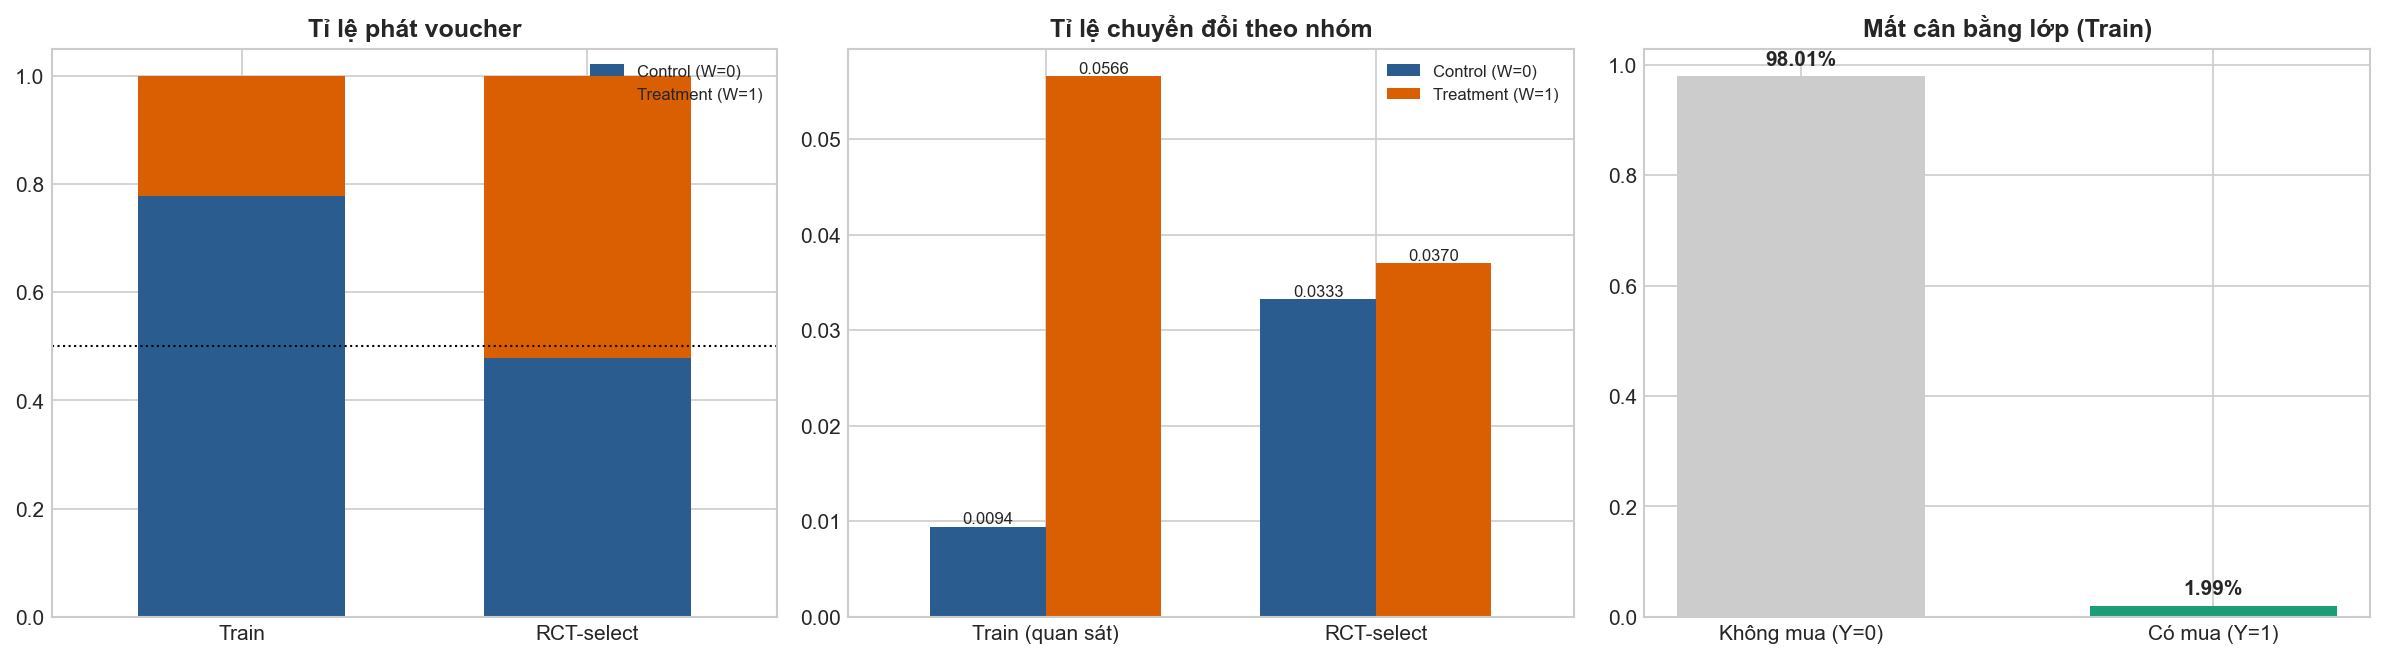
\includegraphics[width=\textwidth]{treatment-outcome.png}
    \caption{So sánh cơ chế treatment, tỷ lệ chuyển đổi và mức mất cân bằng
    lớp. Dữ liệu quan sát chỉ có $22.17\%$ khách nhận voucher và tỷ lệ mua
    toàn tập khoảng $1.99\%$; RCT có treatment gần $50\%$ theo thiết kế.}
    \label{fig:treatment-outcome}
\end{figure}

\subsection{Đo lường thiên vị chọn lọc bằng chỉ số SMD}
Chỉ số \textbf{Standardized Mean Difference (SMD)} được dùng để đo mức
chênh lệch giữa nhóm $T=1$ và $T=0$ trên từng đặc trưng $X_j$:
\[
\operatorname{SMD}(X_j)=
\frac{\bar{X}_{j,T=1}-\bar{X}_{j,T=0}}
{\sqrt{\left(s_{j,T=1}^2+s_{j,T=0}^2\right)/2}}.
\]
Ngưỡng thường dùng để cảnh báo mất cân bằng là
$\lvert\operatorname{SMD}\rvert>0.1$. Dữ liệu quan sát có nhiều đặc trưng
vượt ngưỡng này, trong khi SMD của RCT tập trung gần 0 hơn.

\begin{table}[H]
\centering
\small
\begin{tabularx}{\textwidth}{>{\raggedright\arraybackslash}p{4.4cm}X}
\toprule
\textbf{Chẩn đoán} & \textbf{Kết quả trên dữ liệu dự án} \\
\midrule
Quy mô nguồn dữ liệu & $926\,669$ quan sát lịch sử và $181\,669$ quan sát RCT. \\
Tỷ lệ treatment & $22.17\%$ trên \code{train}, so với $52.12\%$ trên \code{RCT-select}. \\
Mất cân bằng covariate & \textbf{46/74} đặc trưng được chẩn đoán ở bước EDA trên \code{train} có $|\mathrm{SMD}|>0.25$; lớn nhất $0.911$ ở \code{f9}. \\
Kiểm chứng ngẫu nhiên hóa & $|\mathrm{SMD}|$ lớn nhất trên \code{RCT-select} chỉ $0.054$. \\
Chênh lệch chuyển đổi thô & $4.719\pp$ trên dữ liệu quan sát, so với hiệu ứng $0.372\pp$ đo trên RCT: cao gấp $12.7$ lần. \\
Khả năng phân biệt treatment & Propensity model đạt ROC--AUC $0.9322$, cho thấy cơ chế phát voucher lịch sử phụ thuộc mạnh vào $X$. \\
\bottomrule
\end{tabularx}
\caption{Chẩn đoán thiên vị chọn lọc trên \code{train} và kiểm chứng cân bằng
trên \code{RCT-select}. Chênh lệch chuyển đổi thô của dữ liệu quan sát không
được diễn giải như tác động nhân quả.}
\label{tab:bias-diagnostics}
\end{table}

Bảng~\ref{tab:bias-diagnostics} cho thấy vấn đề không chỉ nằm ở quy mô hai
nguồn dữ liệu. Treatment trong dữ liệu lịch sử có thể được dự đoán rất tốt từ
covariate, nên nhóm nhận và không nhận voucher vốn đã khác nhau trước can
thiệp. Hình~\ref{fig:bias-diagnostics} trực quan hóa hệ quả của khác biệt này.

\begin{figure}[H]
    \centering
    \begin{subfigure}[b]{0.47\textwidth}
        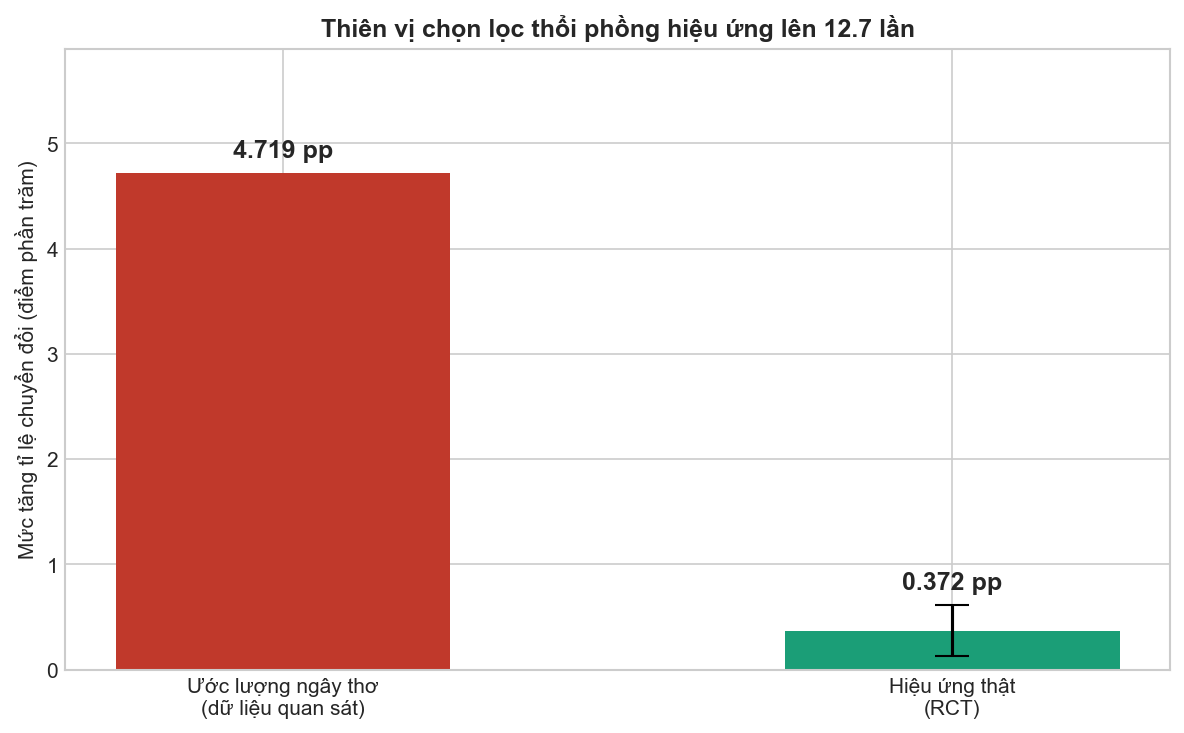
\includegraphics[width=\textwidth]{fig-bias.png}
        \caption{Chênh lệch thô so với hiệu ứng RCT}
    \end{subfigure}\hfill
    \begin{subfigure}[b]{0.51\textwidth}
        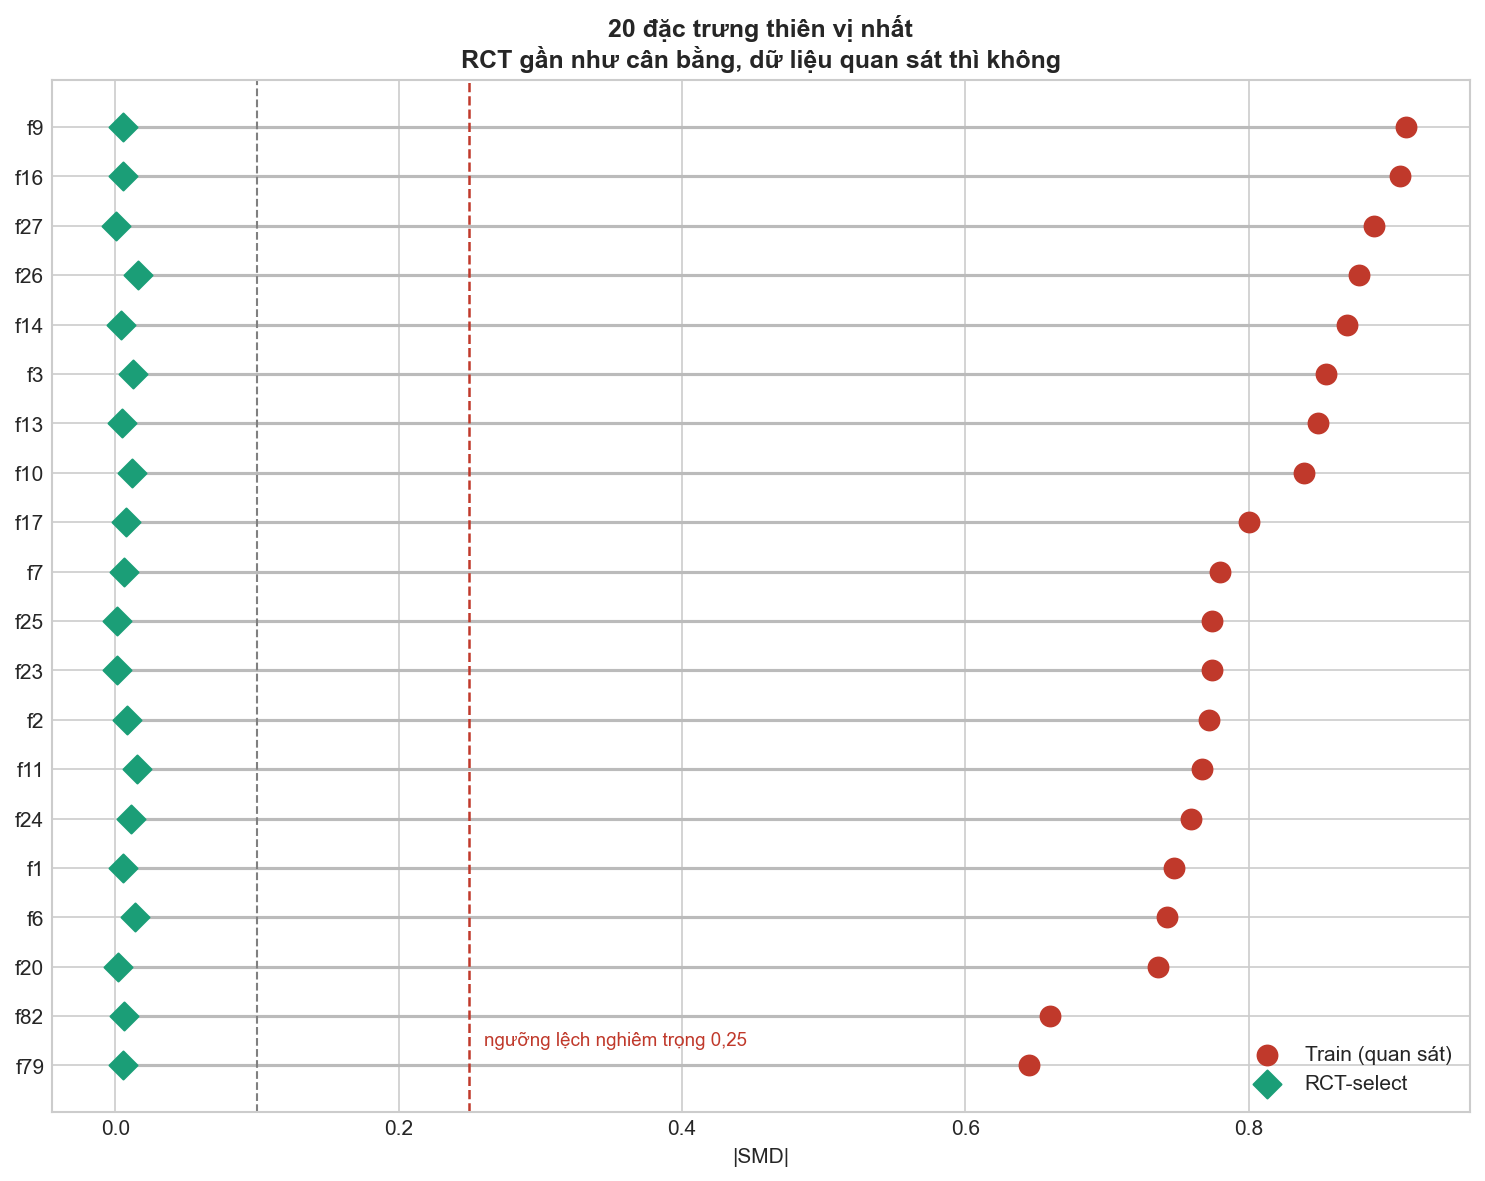
\includegraphics[width=\textwidth]{fig-love.png}
        \caption{Love plot của 20 đặc trưng lệch nhất}
    \end{subfigure}
    \caption{Chẩn đoán thiên vị chọn lọc. Dữ liệu quan sát thổi phồng mức
    tăng conversion từ $0.372\pp$ lên $4.719\pp$. Đồng thời, nhiều đặc trưng
    vượt xa ngưỡng lệch nghiêm trọng $0.25$, trong khi cùng các đặc trưng đó
    gần cân bằng trên RCT.}
    \label{fig:bias-diagnostics}
\end{figure}

\begin{figure}[H]
    \centering
    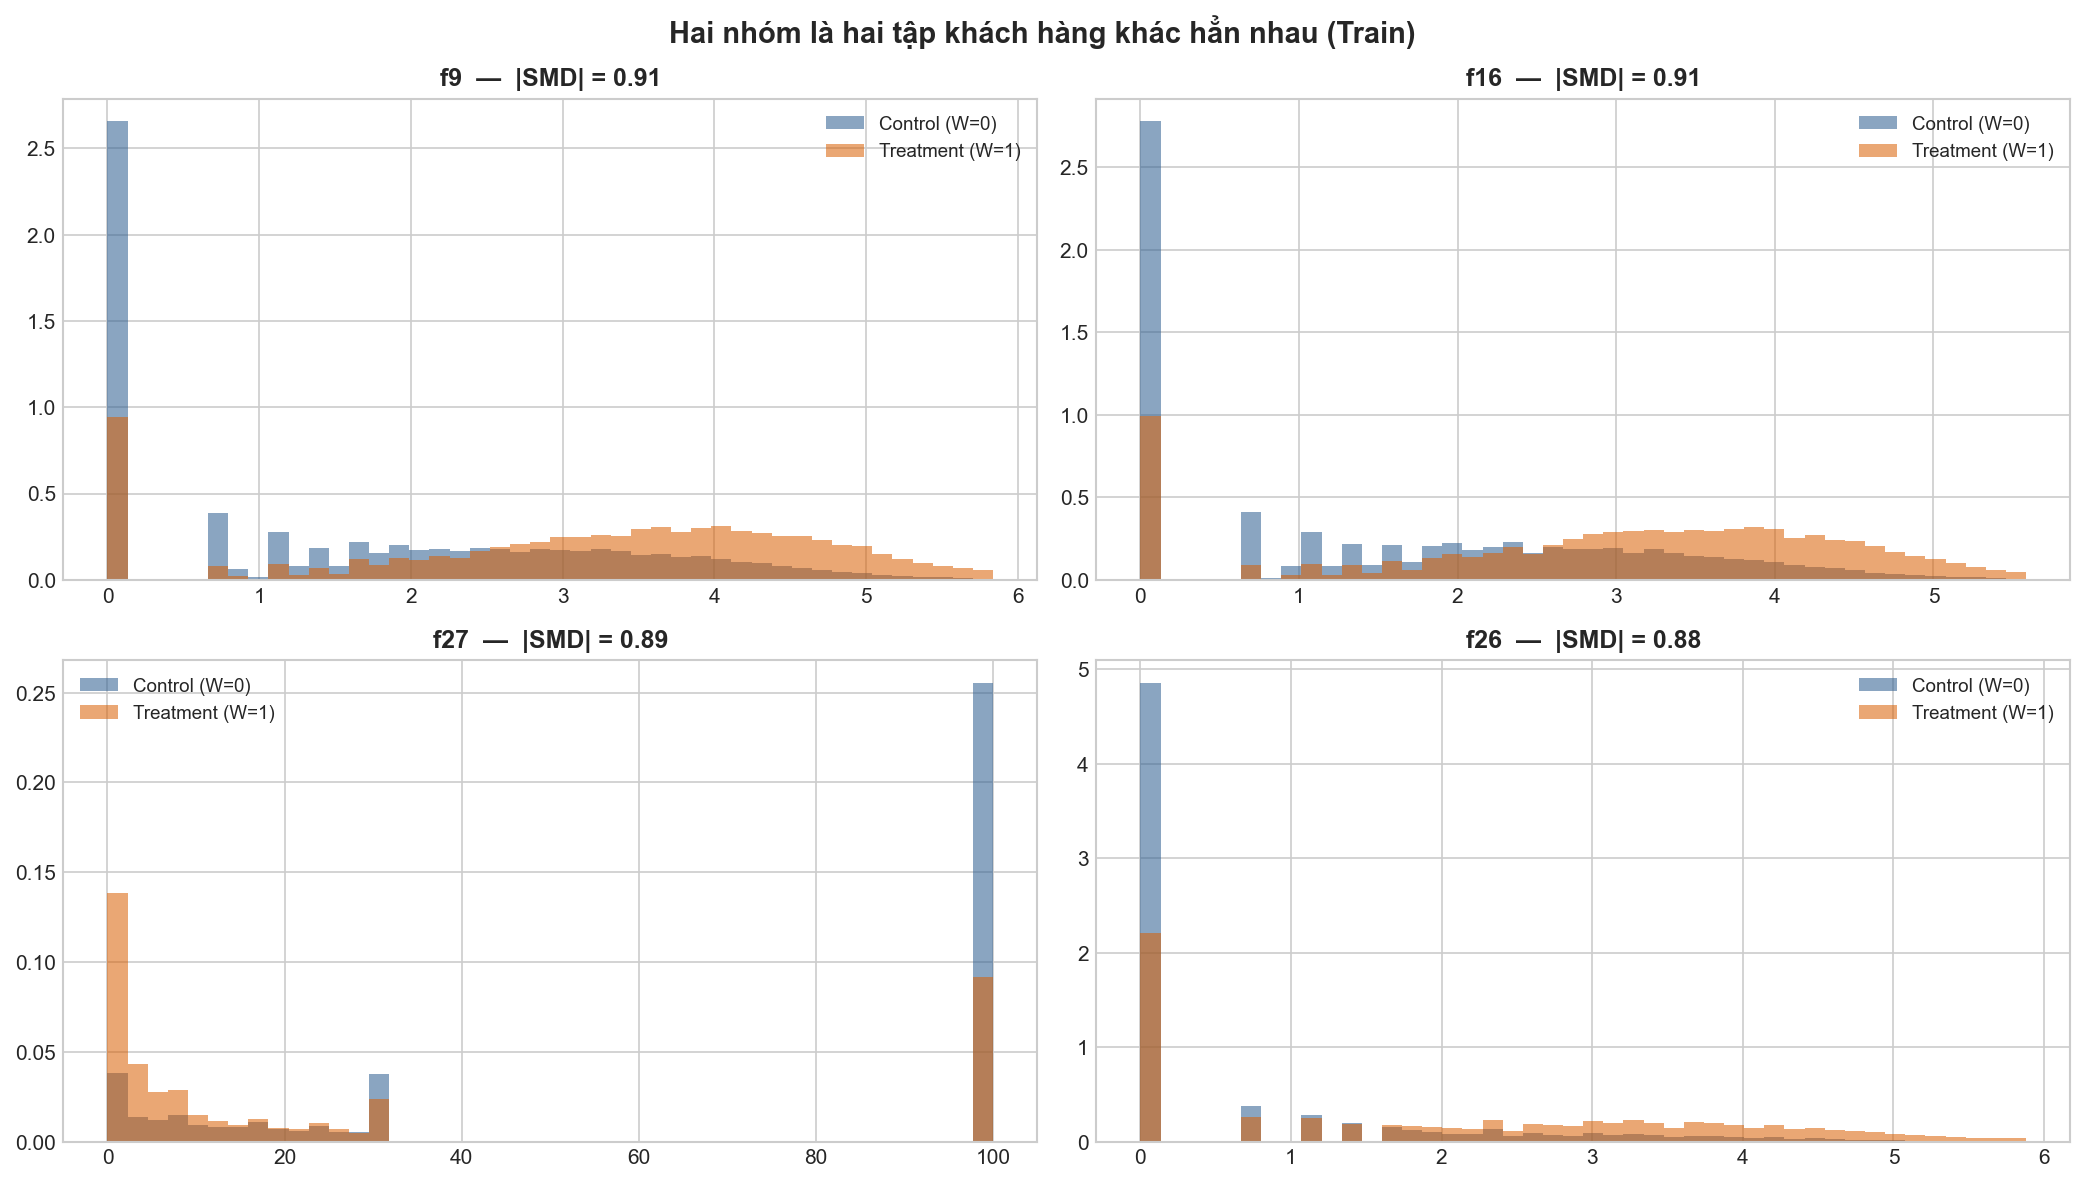
\includegraphics[width=0.96\textwidth]{bias-top4.png}
    \caption{Phân phối treatment--control của bốn đặc trưng có SMD lớn nhất
    trên \code{train}. Khác biệt không chỉ nằm ở trung bình mà xuất hiện trên
    toàn bộ hình dạng phân phối, cho thấy hai nhóm lịch sử là hai quần thể
    khách hàng khác nhau đáng kể.}
    \label{fig:bias-top4}
\end{figure}

\begin{figure}[H]
    \centering
    \begin{subfigure}[b]{0.98\textwidth}
        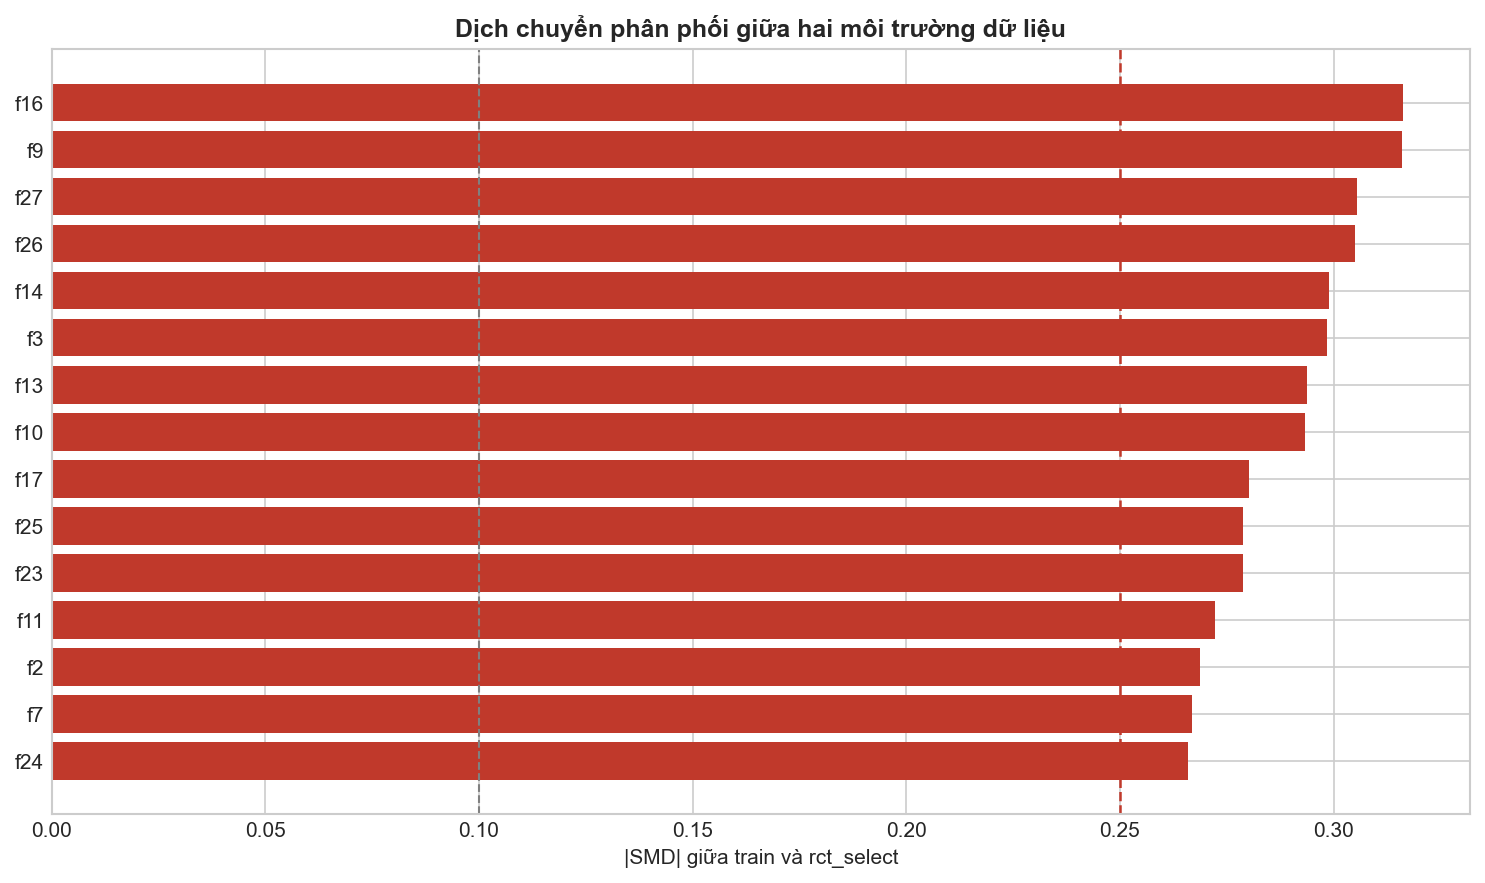
\includegraphics[width=\textwidth]{covariate-shift.png}
        \caption{SMD giữa \code{train} và \code{RCT-select}}
    \end{subfigure}

    \vspace{0.6em}
    \begin{subfigure}[b]{0.98\textwidth}
        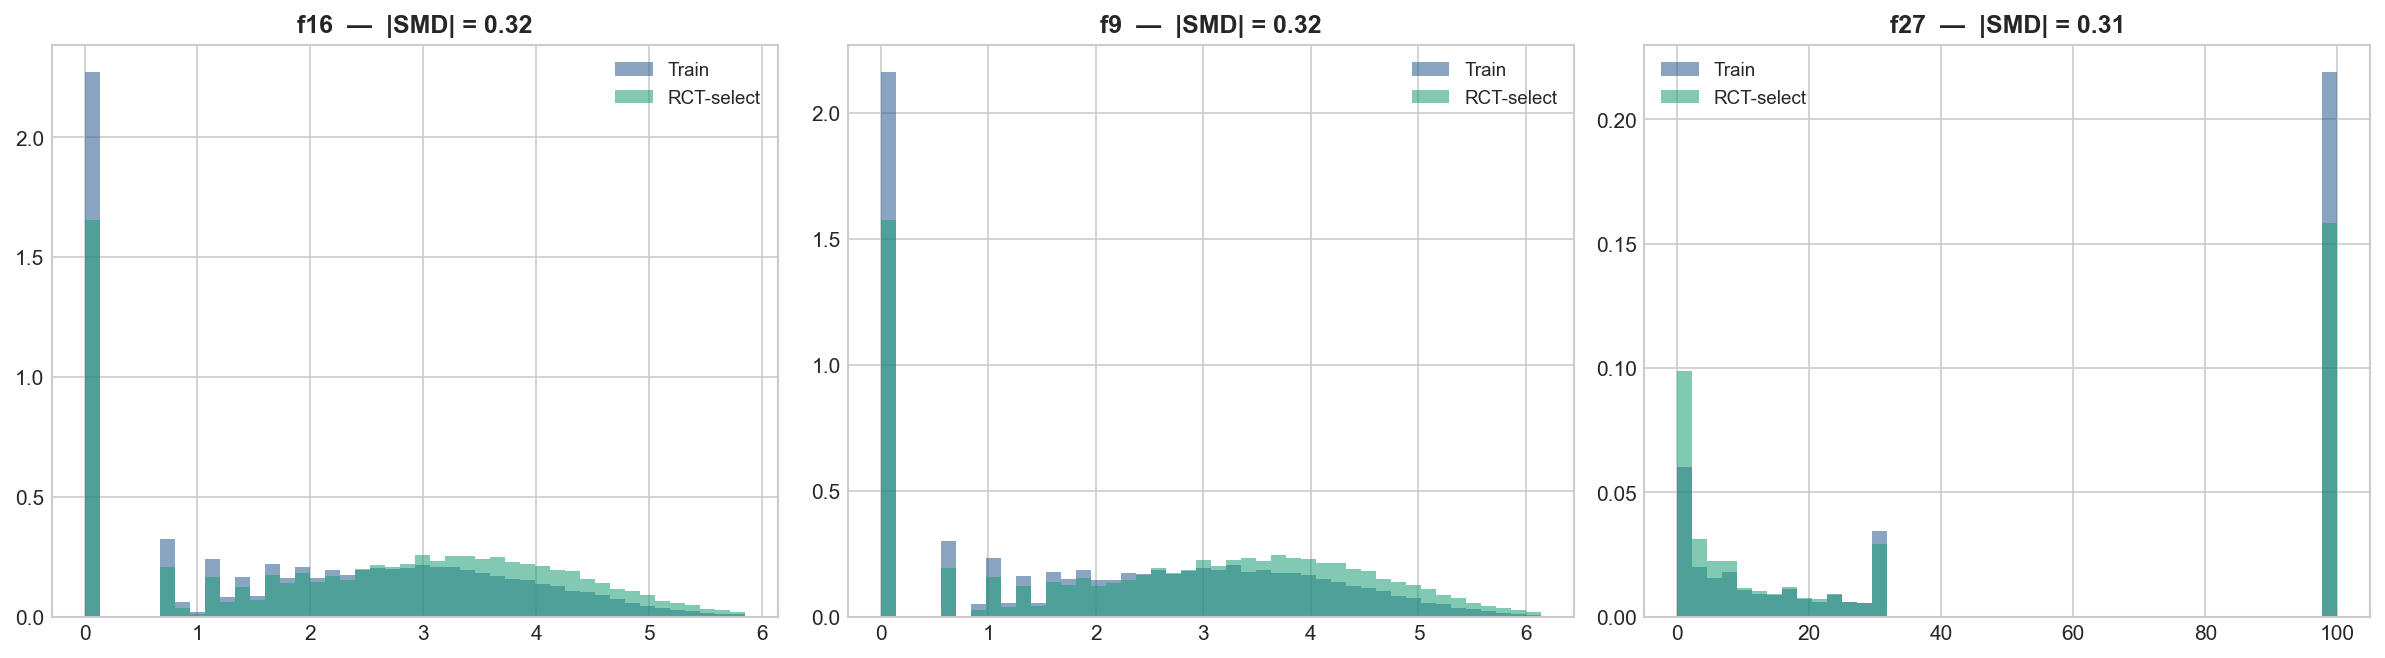
\includegraphics[width=\textwidth]{train-rct-distributions.png}
        \caption{Phân phối của ba đặc trưng dịch chuyển mạnh nhất}
    \end{subfigure}
    \caption{Chẩn đoán covariate shift giữa môi trường quan sát và RCT.
    Mười tám trong 74 đặc trưng có $|\mathrm{SMD}|>0.25$; vì vậy chất lượng
    trên validation quan sát không bảo đảm được khả năng khái quát sang RCT.}
    \label{fig:covariate-shift}
\end{figure}

\begin{figure}[H]
    \centering
    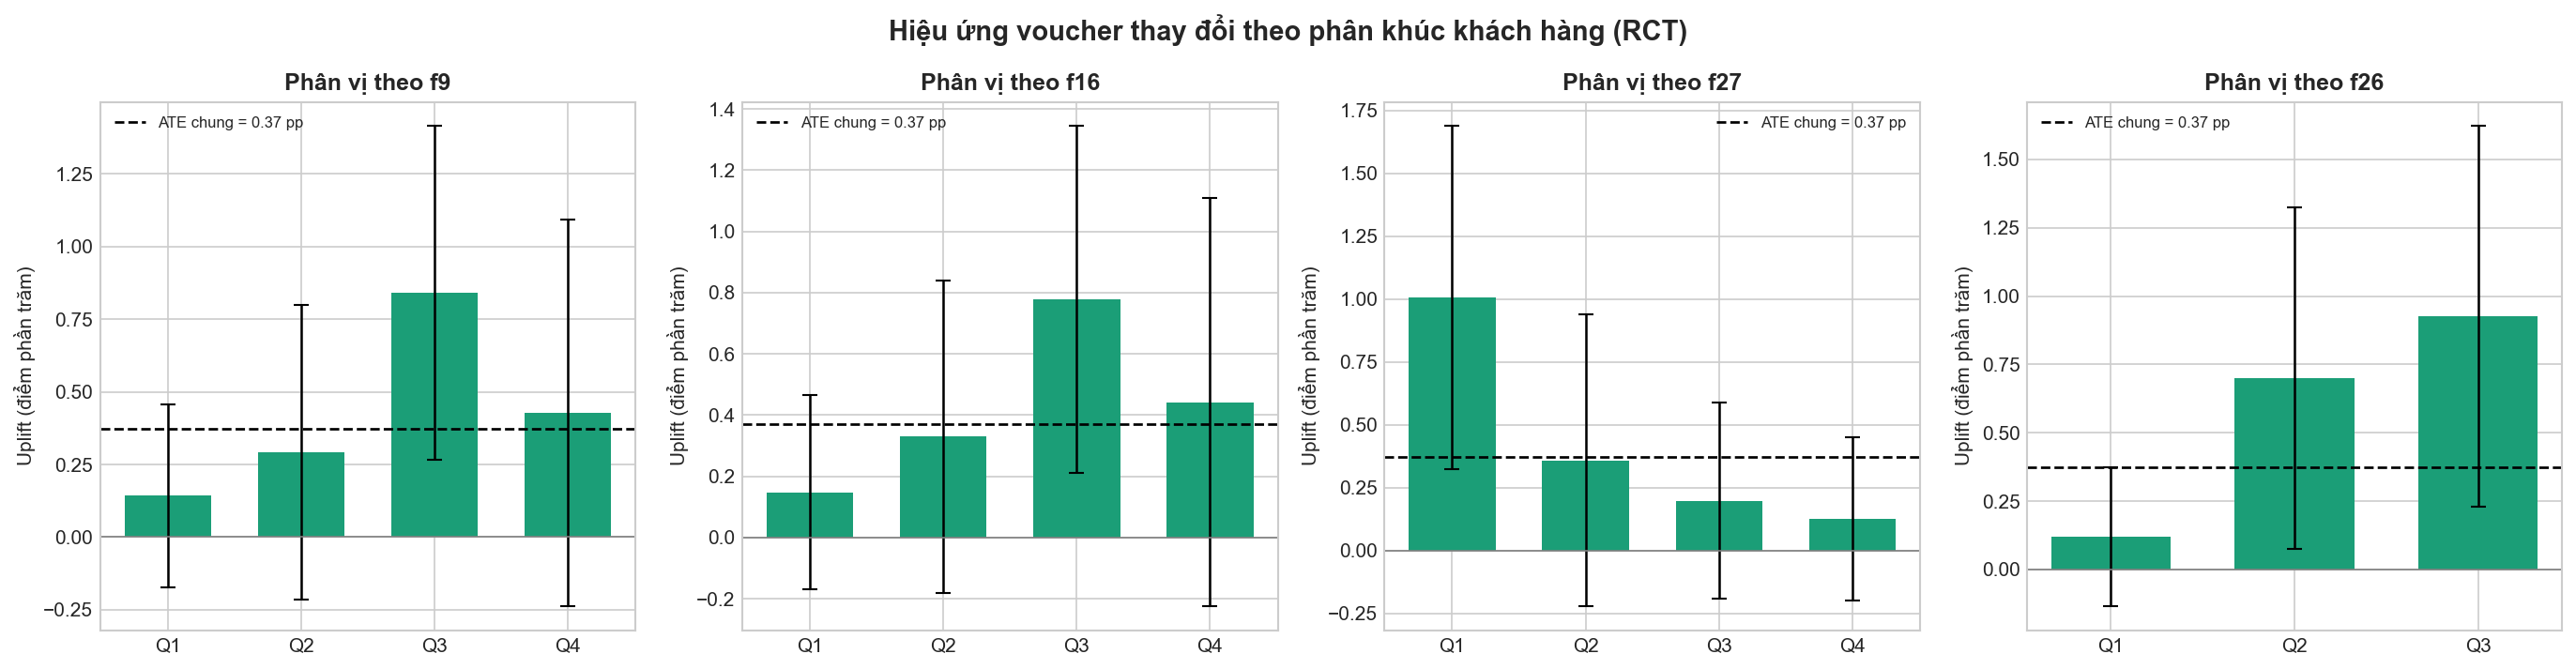
\includegraphics[width=\textwidth]{segment-uplift.png}
    \caption{Uplift đo trực tiếp trên RCT theo các phân vị của bốn đặc trưng.
    Các cột thể hiện chênh lệch conversion treatment--control, thanh lỗi là
    KTC 95\% và đường đứt là ATE toàn RCT. Đây là bằng chứng mô tả về hiệu
    ứng không đồng nhất, không phải kết quả chọn feature cho mô hình.}
    \label{fig:segment-uplift}
\end{figure}

\subsection{Các giả định suy luận nhân quả cốt lõi}
Để nhận dạng CATE từ dữ liệu quan sát, nghiên cứu dựa trên các giả định sau:
\begin{enumerate}
    \item \textbf{Consistency và SUTVA:} treatment được định nghĩa nhất quán,
    không có nhiều phiên bản treatment không được mô hình hóa, và kết quả của
    một khách hàng không bị ảnh hưởng bởi treatment của khách hàng khác.
    \item \textbf{Conditional exchangeability (unconfoundedness):}
    $(Y^{(1)},Y^{(0)})\indep T\mid X$. Sau khi điều kiện hóa theo $X$, không
    còn biến nhiễu chung chưa quan sát giữa treatment và outcome.
    \item \textbf{Overlap/positivity:} tồn tại $\eta>0$ sao cho
    $\eta\le e(X)\le 1-\eta$ trên quần thể mục tiêu.
\end{enumerate}

\begin{figure}[H]
    \centering
    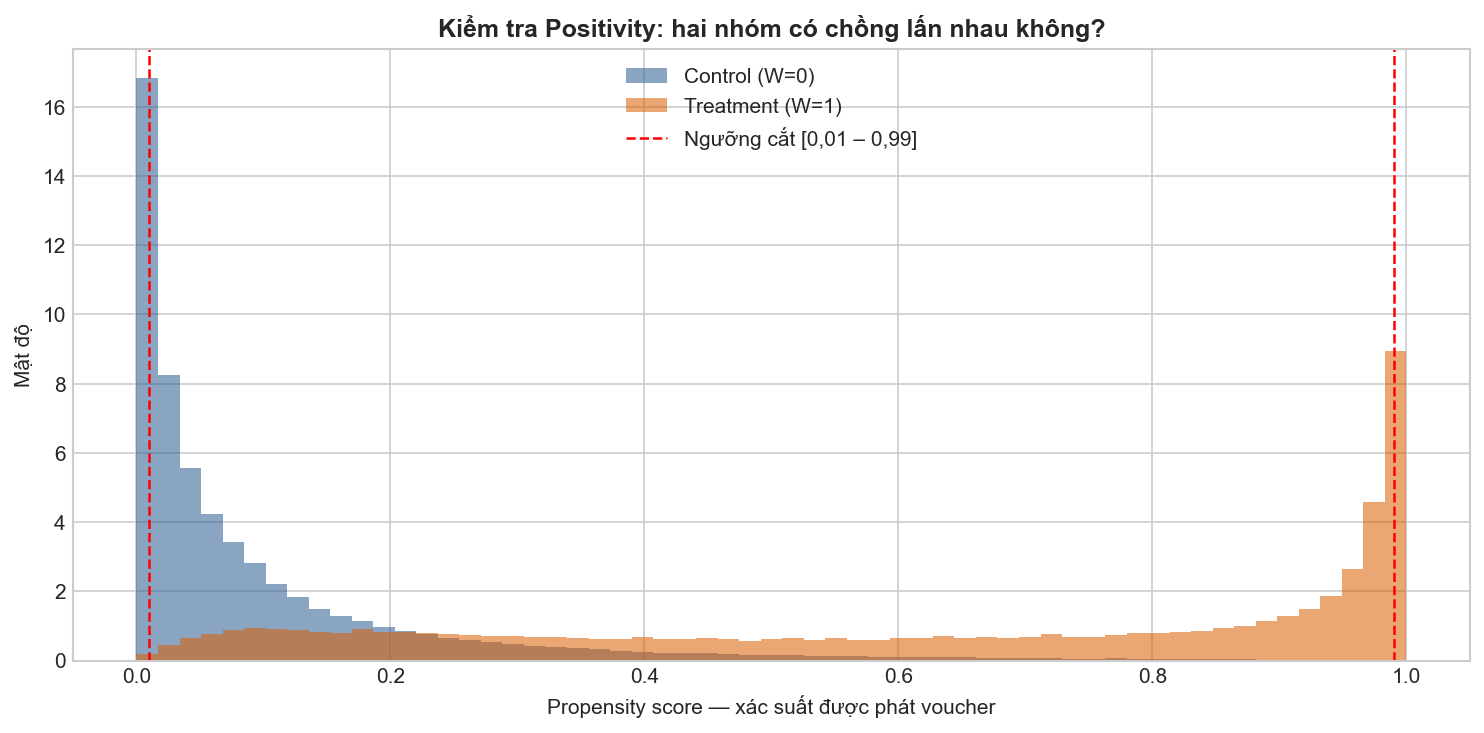
\includegraphics[width=0.9\textwidth]{propensity-overlap.png}
    \caption{Phân phối propensity score trên dữ liệu quan sát. Hai nhóm vẫn
    có vùng chồng lấn, nhưng khối lượng lớn tập trung gần 0 và 1; các vạch đỏ
    biểu diễn ngưỡng chẩn đoán $[0.01,\,0.99]$. Điều này giải thích vì sao
    cần clip/trim trước khi dùng pseudo-outcome doubly robust.}
    \label{fig:propensity-overlap}
\end{figure}

\section{Cơ chế hoạt động của các mô hình CATE}

Nghiên cứu tiến hành cài đặt và so sánh 6 họ mô hình ước lượng CATE:

\begin{table}[H]
\centering
\small
\begin{tabularx}{\textwidth}{>{\raggedright\arraybackslash}p{3.0cm}
    >{\raggedright\arraybackslash}p{2.6cm}X}
\toprule
\textbf{Ước lượng} & \textbf{Nhóm} & \textbf{Nguyên lý chính} \\
\midrule
S-Learner & Meta-learner & Một outcome model coi treatment như một feature; lấy hiệu hai dự đoán khi đặt $T=1$ và $T=0$. \\
T-Learner & Meta-learner & Hai outcome model độc lập cho treatment và control; CATE là hiệu hai bề mặt dự đoán. \\
DR-Learner & Doubly robust & Cross-fitting nuisance model, dựng pseudo-outcome doubly robust rồi hồi quy lên $X$. \\
LinearDML & DML & Khử phần dư treatment/outcome rồi dùng tầng cuối tuyến tính. \\
NonParamDML & DML & Giữ bước khử phần dư nhưng dùng tầng cuối phi tham số linh hoạt hơn. \\
CausalForestDML & DML + causal forest & Dùng causal forest với honest splitting ở tầng cuối để mô hình hóa dị biệt hiệu ứng. \\
\bottomrule
\end{tabularx}
\caption{Sáu họ ước lượng CATE được benchmark. Đây là sáu giả định mô hình
khác nhau, không phải sáu cấu hình của cùng một thuật toán.}
\label{tab:cate-estimators}
\end{table}

\subsection{Nhóm mô hình cơ sở}

\subsubsection{S-Learner (Single Learner)}
S-Learner sử dụng \textbf{một mô hình học máy} $\mu(X,T)$ để dự đoán $Y$,
trong đó treatment $T$ được đưa vào như một đặc trưng:
\[
\hat{\tau}_{S}(X)=\hat{\mu}(X,T=1)-\hat{\mu}(X,T=0).
\]
\begin{itemize}
    \item \textbf{Ưu điểm:} Đơn giản và tận dụng toàn bộ dữ liệu trong một mô hình.
    \item \textbf{Hạn chế:} Khi tín hiệu treatment yếu hoặc không gian đặc
    trưng lớn, regularization có thể khiến mô hình ít sử dụng $T$, làm co
    ước lượng hiệu ứng về 0.
\end{itemize}

\subsubsection{T-Learner (Two Learners)}
T-Learner huấn luyện hai mô hình outcome riêng theo treatment:
\[
\hat{\mu}_1(X)=\operatorname{Model}_1(Y\mid X,T=1),\qquad
\hat{\mu}_0(X)=\operatorname{Model}_0(Y\mid X,T=0),
\]
\[
\hat{\tau}_{T}(X)=\hat{\mu}_1(X)-\hat{\mu}_0(X).
\]
\begin{itemize}
    \item \textbf{Ưu điểm:} Cho phép hai bề mặt outcome khác nhau giữa hai nhóm.
    \item \textbf{Hạn chế:} Nếu hai nhóm mất cân bằng hoặc overlap kém, mô
    hình ở vùng ít dữ liệu có phương sai và sai số ngoại suy cao; sai số của
    cả hai outcome model cùng truyền vào hiệu số CATE.
\end{itemize}

\subsection{Họ mô hình DR-Learner}

DR-Learner là phương pháp hai giai đoạn dựa trên pseudo-outcome doubly
robust \cite{kennedy2020,robins1994}.

\subsubsection{Quy trình ước lượng}
\begin{enumerate}
\item \textbf{Ước lượng nuisance:} Dùng cross-fitting $K$-fold để ước lượng
propensity score $\hat e(X)=\Prob(T=1\mid X)$ và hai outcome regression
$\hat\mu_1(X)=\Exp[Y\mid T=1,X]$, $\hat\mu_0(X)=\Exp[Y\mid T=0,X]$.
\item \textbf{Tạo pseudo-outcome:}
\begin{equation}
\tilde{Y}_i = \hat{\mu}_1(X_i) - \hat{\mu}_0(X_i)
+ \frac{T_i\{Y_i - \hat{\mu}_1(X_i)\}}{\hat{e}(X_i)}
- \frac{(1-T_i)\{Y_i - \hat{\mu}_0(X_i)\}}{1 - \hat{e}(X_i)}.
\end{equation}
\item \textbf{Hồi quy CATE cuối:} Hồi quy $\tilde Y$ theo $X$, chẳng hạn
bằng LightGBM:
\[
\hat{\tau}_{DR}(X)=\operatorname{Regress}(\tilde{Y}\mid X).
\]
\end{enumerate}

\subsubsection{Tính chất doubly robust}

\begin{theorem}[Doubly Robust Property]
Dưới consistency, conditional exchangeability và positivity, kỳ vọng điều
kiện $\Exp[\tilde{Y}\mid X]$ bằng CATE $\tau(X)$ nếu ít nhất một trong hai
thành phần nuisance sau được đặc tả đúng: outcome regression $\mu_t(X)$ hoặc
propensity score $e(X)$.
\end{theorem}

\begin{proof}
Xét hai trường hợp độc lập:

\paragraph{Trường hợp 1: outcome model đúng, propensity model sai.}
Khi outcome model đúng, phần dư có kỳ vọng điều kiện bằng 0:
\[
\Exp[Y-\mu_1(X)\mid T=1,X]=0,\qquad
\Exp[Y-\mu_0(X)\mid T=0,X]=0.
\]
Với mọi ước lượng propensity dương $\hat e^*(X)$, ta có
\begin{align*}
\Exp[\tilde{Y}\mid X]
&=\mu_1(X)-\mu_0(X)
+\frac{\Exp[T\{Y-\mu_1(X)\}\mid X]}{\hat e^*(X)}
-\frac{\Exp[(1-T)\{Y-\mu_0(X)\}\mid X]}{1-\hat e^*(X)}\\
&=\mu_1(X)-\mu_0(X)=\tau(X).
\end{align*}
Hai số hạng hiệu chỉnh có kỳ vọng bằng 0 dù propensity model bị đặc tả sai.

\paragraph{Trường hợp 2: propensity model đúng, outcome model sai.}
Gọi $\mu_t^*(X)$ là outcome model có thể bị đặc tả sai. Khi propensity model
đúng, conditional exchangeability cho
\[
\Exp\left[\frac{T\{Y-\mu_1^*(X)\}}{e(X)}\,\middle|\,X\right]
=\mu_1(X)-\mu_1^*(X),
\]
và tương tự cho nhóm control. Do đó
\begin{align*}
\Exp[\tilde{Y}\mid X]
&=\mu_1^*(X)-\mu_0^*(X)
+\{\mu_1(X)-\mu_1^*(X)\}
-\{\mu_0(X)-\mu_0^*(X)\}\\
&=\mu_1(X)-\mu_0(X)=\tau(X).
\end{align*}
Sai số của outcome model được bù bởi hai số hạng hiệu chỉnh khi propensity
model đúng.
\end{proof}

\subsection{Họ mô hình Double Machine Learning}

DML giảm ảnh hưởng bậc nhất của sai số ước lượng nuisance bằng Neyman
orthogonality và cross-fitting \cite{chernozhukov2018}.

\subsubsection{Nguyên lý partialling-out}
Với treatment nhị phân và mô hình outcome có điều kiện
$\Exp[Y\mid X,T]=\mu_0(X)+T\tau(X)$, đặt
$m(X)=\Exp[Y\mid X]$ và $e(X)=\Exp[T\mid X]$. Khi đó
\[
Y-m(X)=\tau(X)\{T-e(X)\}+\varepsilon,
\qquad \Exp[\varepsilon\mid X,T]=0.
\]
Trong thực nghiệm, các phần dư được xây dựng từ dự đoán ngoài fold:
$\tilde Y_{res}=Y-\hat m(X)$ và $\tilde T_{res}=T-\hat e(X)$.

\subsubsection{Các biến thể DML trong nghiên cứu}
\begin{itemize}
    \item \textbf{LinearDML:} Mô hình hóa CATE theo dạng tuyến tính
    $\tau(X)=X^\top\theta$.
    \item \textbf{NonParamDML:} Cho phép final stage phi tham số để biểu diễn
    bề mặt CATE linh hoạt hơn.
    \item \textbf{CausalForestDML:} Dùng causal forest với honest splitting.
    Khoảng tin cậy chỉ có diễn giải thống kê hợp lệ khi các giả định và điều
    kiện tiệm cận của phương pháp được đáp ứng.
\end{itemize}

\section{Quy trình thực nghiệm Data Science}

Dự án thiết kế luồng xử lý 4 Notebooks tuần tự, nối với nhau qua tệp Parquet và JSON:

\subsection{Notebook 01: \code{01\_eda.ipynb} --- phân tích và chia dữ liệu}
\begin{itemize}
    \item Phát hiện và loại bỏ các cột hằng số và trùng lặp.
    \item Thiết kế phép chia phân tầng cố định thành bốn tập:
\end{itemize}

\begin{table}[H]
\centering
\small
\begin{tabularx}{\textwidth}{>{\raggedright\arraybackslash}p{2.6cm}
    >{\raggedleft\arraybackslash}p{2.0cm}
    >{\centering\arraybackslash}p{2.0cm}
    >{\centering\arraybackslash}p{1.8cm}X}
\toprule
\textbf{Tập} & \textbf{Số dòng} & \textbf{Treatment} & \textbf{CVR} & \textbf{Vai trò} \\
\midrule
\code{train} & $741\,335$ & $22.17\%$ & $1.99\%$ & Huấn luyện mô hình và nuisance model. \\
\code{val} & $185\,334$ & $22.17\%$ & $1.99\%$ & Tinh chỉnh siêu tham số theo DR-AUUC. \\
\code{RCT-select} & $90\,834$ & $52.12\%$ & $3.52\%$ & Chọn đúng một họ mô hình cuối. \\
\code{RCT-holdout} & $90\,835$ & $52.12\%$ & $3.52\%$ & Đánh giá cuối, mở đúng một lần. \\
\bottomrule
\end{tabularx}
\caption{Bốn tập dữ liệu và vai trò được ấn định trước khi chạy thực nghiệm.}
\label{tab:data-splits}
\end{table}

\begin{figure}[H]
    \centering
    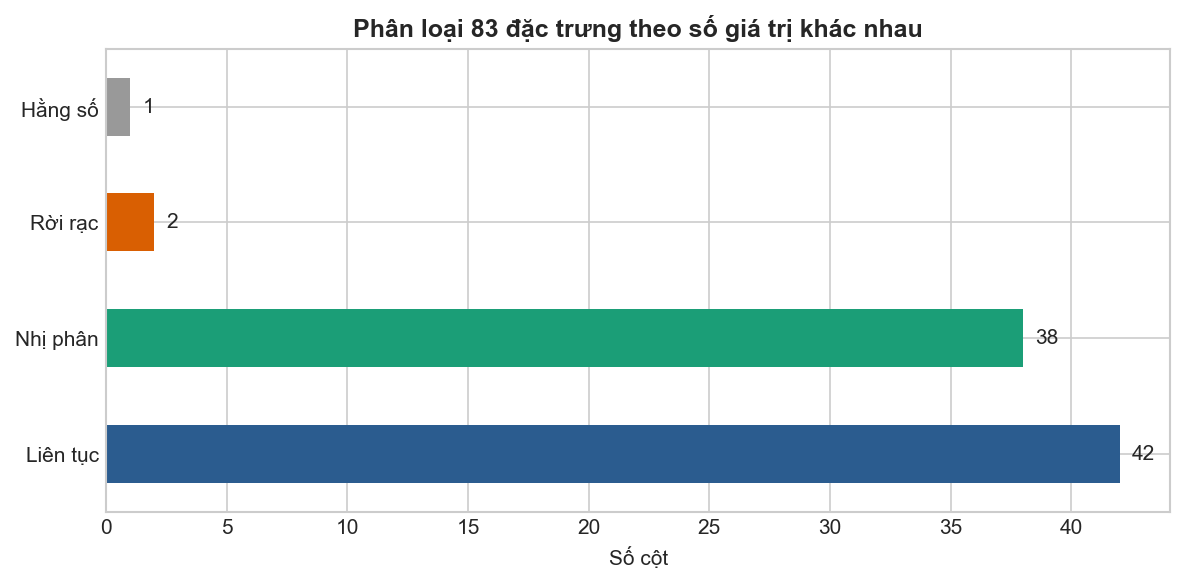
\includegraphics[width=0.78\textwidth]{data-types.png}
    \caption{Phân loại 83 cột ban đầu theo số giá trị khác nhau. Một cột hằng
    được loại ở bước EDA; các cột nhị phân và liên tục chiếm phần lớn không
    gian đặc trưng.}
    \label{fig:data-types}
\end{figure}

\begin{summarybox}[Nguyên tắc sử dụng tập RCT-holdout]
Tập \code{RCT-holdout} bị khóa hoàn toàn trong suốt quá trình phát triển mô
hình. Mọi quyết định về siêu tham số, chọn mô hình hay rút gọn đặc trưng đều
phải hoàn tất trước khi mở tập này.
\end{summarybox}

\subsection{Notebook 02: \code{02\_feature\_engineering.ipynb} --- kỹ nghệ đặc trưng}
Tạo 7 đặc trưng dẫn xuất từ dữ liệu lịch sử. Sau bước làm sạch, đầu vào mô
hình gồm \textbf{76 đặc trưng}: 69 cột gốc và 7 cột dẫn xuất.

\begin{table}[H]
\centering
\scriptsize
\begin{tabularx}{\textwidth}{>{\raggedright\arraybackslash}p{3.5cm}X
    >{\raggedleft\arraybackslash}p{1.7cm}
    >{\raggedleft\arraybackslash}p{1.2cm}}
\toprule
\textbf{Đặc trưng dẫn xuất} & \textbf{Công thức} & \textbf{Mặc định} & \textbf{Hạng gain} \\
\midrule
\code{fe\_ratio\_f1\_f2} & $f_1/(f_2+1)$ & $0.9944$ & 8 \\
\code{fe\_ratio\_f14\_f16} & $f_{14}/(f_{16}+1)$ & $0.0000$ & 29 \\
\code{fe\_ratio\_f9\_f27} & $f_9/(f_{27}+1)$ & $0.0339$ & 6 \\
\code{fe\_inter\_f9\_f26} & $f_9\times f_{26}$ & $0.0000$ & 13 \\
\code{fe\_inter\_f14\_f27} & $f_{14}\times f_{27}$ & $0.0000$ & 44 \\
\code{fe\_nonzero\_top10} & Số cột khác 0 trong nhóm 10 đặc trưng thiên lệch nhất. & $7.0$ & 41 \\
\code{fe\_flag\_sum} & $f_{66}+f_{68}+f_{75}$ & $3.0$ & 50 \\
\bottomrule
\end{tabularx}
\caption{Bảy đặc trưng dẫn xuất, giá trị mặc định và thứ hạng gain trong
model cuối. Bốn đặc trưng dẫn xuất nằm trong top 30 theo gain.}
\label{tab:derived-features}
\end{table}

\begin{figure}[H]
    \centering
    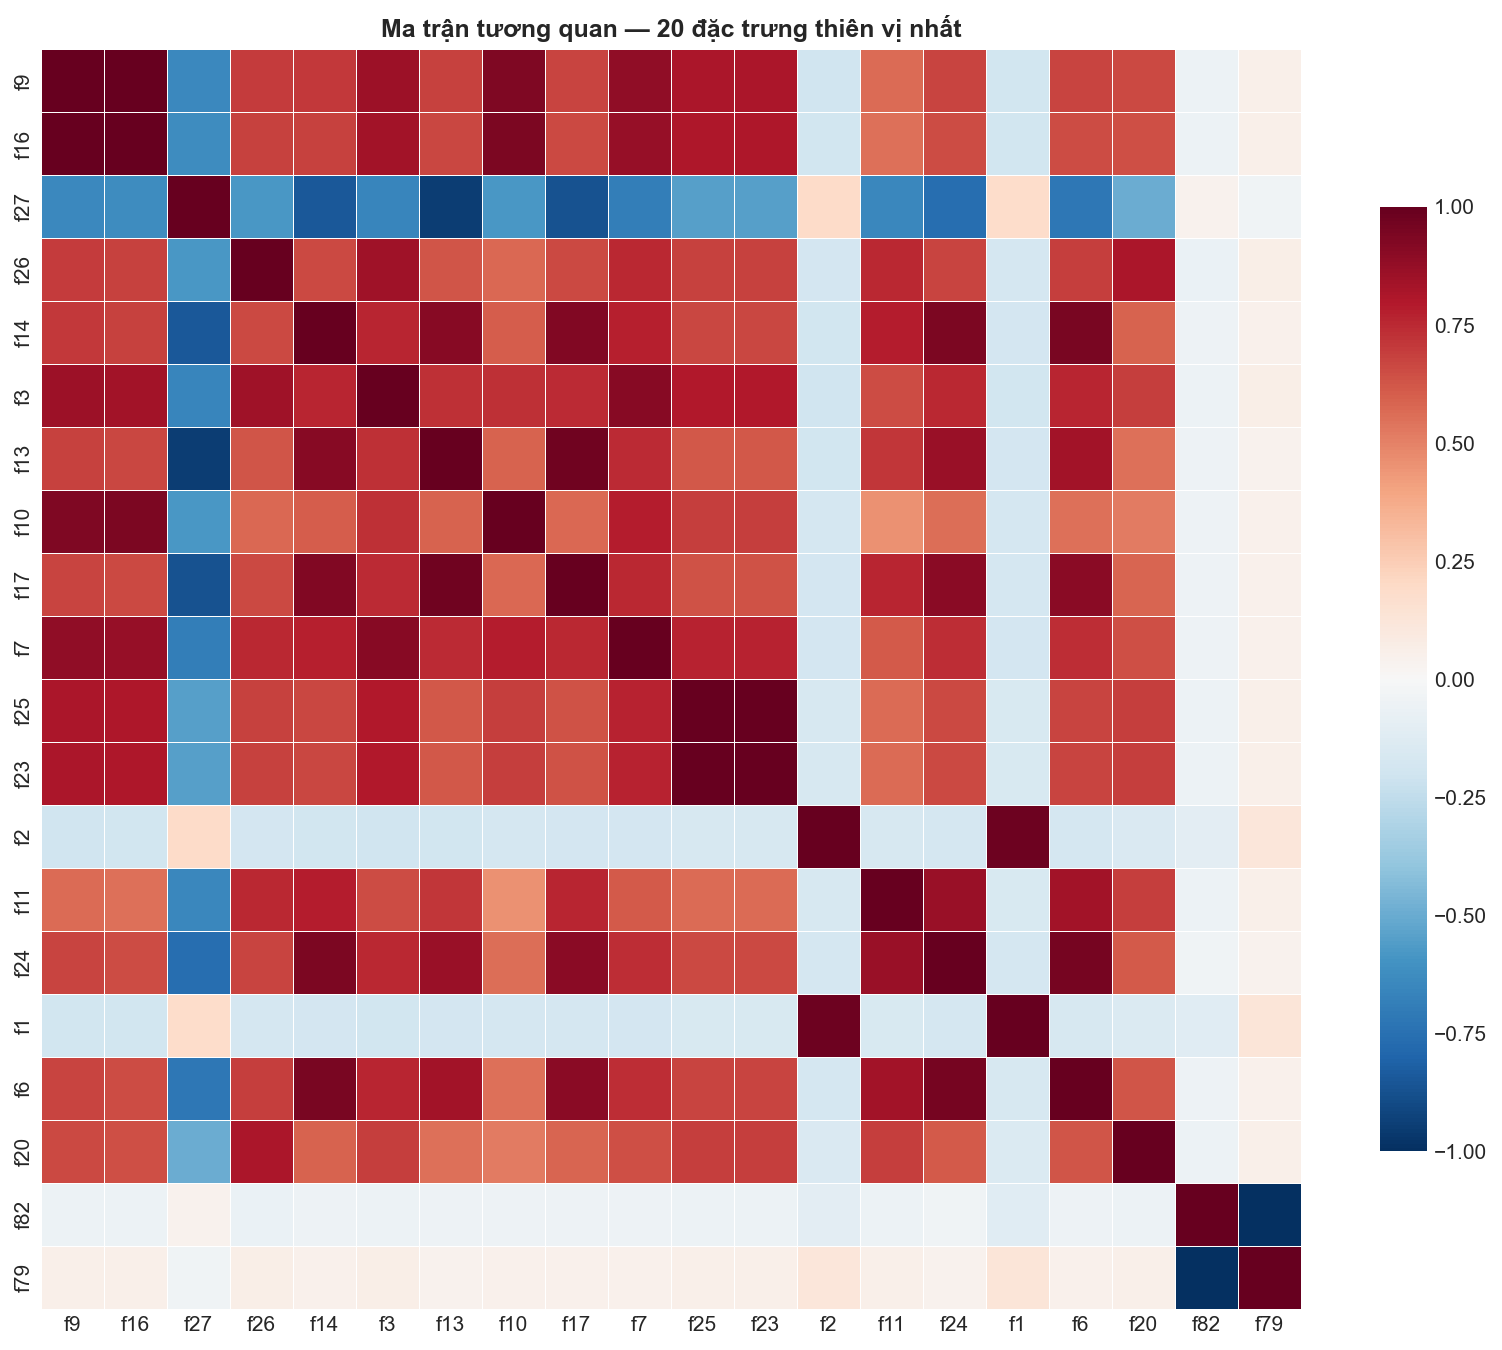
\includegraphics[width=0.76\textwidth]{correlation-heatmap.png}
    \caption{Ma trận tương quan của 20 đặc trưng có selection bias lớn nhất.
    Nhiều cột tạo thành các cụm tương quan mạnh; bước kỹ nghệ vì vậy bổ sung
    ratio, interaction và count thay vì xem từng cột hoàn toàn độc lập.}
    \label{fig:correlation-heatmap}
\end{figure}

\subsection{Notebook 03: \code{03\_model\_tuning.ipynb} --- tuning và overlap}
\begin{itemize}
    \item \textbf{Overlap:} Loại khỏi metric các quan sát có $e(X)$ nằm
    ngoài $[\alpha,1-\alpha]$, với $\alpha=0.071$ được xác định theo quy tắc
    Crump và cộng sự \cite{crump2009}. Estimand của metric vì vậy thuộc quần
    thể overlap, không phải toàn bộ tập validation.
    \item \textbf{Winsorization:} Giới hạn pseudo-outcome tại phân vị 0.5\%
    và 99.5\% để ổn định metric xếp hạng; biến đã winsorize không được dùng
    để báo cáo mức ATE.
    \item \textbf{Optuna và MLflow:} Optuna đề xuất siêu tham số cho 66 trial
    trên \code{Val}, tối đa hóa DR-AUUC chuẩn hóa (được lưu với tên
    \code{dr\_qini}). MLflow ghi tham số, metric và thời gian fit của từng
    trial vào SQLite \code{mlflow.db}.
\end{itemize}

\begin{table}[H]
\centering
\scriptsize
\begin{tabular}{@{}lrrrrr@{}}
\toprule
$\alpha$ & \textbf{Giữ lại} & \textbf{Số dòng} &
\textbf{ATE$_{DR}$ clip} & \textbf{ATE$_{DR}$ trim} & $\max|\widetilde Y|$ \\
\midrule
$0.010$ & $81.11\%$ & $81\,114$ & $0.502\pp$ & $0.537\pp$ & $76.10$ \\
$0.020$ & $68.79\%$ & $68\,790$ & $0.551\pp$ & $0.344\pp$ & $34.78$ \\
$0.050$ & $51.35\%$ & $51\,352$ & $0.558\pp$ & $0.328\pp$ & $19.48$ \\
\textbf{$0.071$} & \textbf{$43.32\%$} & \textbf{$43\,323$} & \textbf{$0.581\pp$} & \textbf{$0.493\pp$} & \textbf{$12.44$} \\
$0.100$ & $35.31\%$ & $35\,314$ & $0.624\pp$ & $0.584\pp$ & $9.53$ \\
\bottomrule
\end{tabular}
\caption{Đánh đổi khi quét ngưỡng overlap trên 100.000 dòng validation.
Ngưỡng $\alpha=0.071$ theo quy tắc Crump giữ lại $43.32\%$ dữ liệu và chặn
đuôi pseudo-outcome từ $76.10$ xuống $12.44$.}
\label{tab:overlap-threshold}
\end{table}

\begin{table}[H]
\centering
\small
\begin{tabularx}{0.92\textwidth}{X
    >{\centering\arraybackslash}p{2.1cm}
    >{\centering\arraybackslash}p{3.2cm}}
\toprule
\textbf{Cách ước lượng trên validation} & \textbf{ATE} & \textbf{KTC 95\%} \\
\midrule
Chênh lệch thô -- toàn validation & $4.720\pp$ & Không áp dụng \\
Chênh lệch thô -- vùng overlap & $1.970\pp$ & Không áp dụng \\
Doubly robust -- toàn validation, chỉ clip & $0.581\pp$ & Không báo cáo \\
Doubly robust -- vùng overlap, đã trim & $0.493\pp$ & $[0.155,\,0.832]\pp$ \\
\midrule
Mốc ATE đo trực tiếp trên RCT & $0.372\pp$ & $[0.132,\,0.611]\pp$ \\
\bottomrule
\end{tabularx}
\caption{Tác dụng của hiệu chỉnh doubly robust và overlap trimming. Trên vùng
overlap, hiệu chỉnh kéo ước lượng từ $1.970\pp$ xuống $0.493\pp$, gần mốc
RCT hơn rõ rệt.}
\label{tab:dr-adjustment-ladder}
\end{table}

Trước khi dùng $Qini_{DR}$ làm mục tiêu Optuna, implementation được kiểm tra
bằng các trường hợp biên trong Bảng~\ref{tab:metric-validation}.

\begin{table}[H]
\centering
\small
\begin{tabularx}{\textwidth}{>{\raggedright\arraybackslash}X
    >{\centering\arraybackslash}p{3.6cm}
    >{\centering\arraybackslash}p{3.4cm}}
\toprule
\textbf{Phép kiểm} & \textbf{Validation DR} & \textbf{RCT} \\
\midrule
Xếp hạng biết trước đáp án & $Qini_{DR}=1.0000$ -- đạt & Diện tích gấp $195.5$ lần ngẫu nhiên -- đạt \\
Xếp hạng đảo ngược & $Qini_{DR}=-1.0000$ -- đạt & Không áp dụng \\
Xếp hạng ngẫu nhiên & $0.0006\pm0.0075$ -- đạt & $-0.0051\ [-0.0264,\,0.0150]$ -- đạt \\
Pha nhiễu tăng dần & $1.000\rightarrow0.235$ -- đạt & $1.000\rightarrow0.362$ -- đạt \\
ATE so với phép tính tay & Không áp dụng & Sai lệch $0.0\mathrm{e}{+00}$ -- đạt \\
\bottomrule
\end{tabularx}
\caption{Kiểm chứng thước đo trước khi sử dụng trong tuning và benchmark.
Các phép thử có assert chốt cổng để metric sai không âm thầm đi tiếp.}
\label{tab:metric-validation}
\end{table}

\begin{table}[H]
\centering
\small
\begin{tabularx}{\textwidth}{>{\raggedright\arraybackslash}X
    >{\centering\arraybackslash}p{1.5cm}
    >{\centering\arraybackslash}p{4.5cm}
    >{\raggedleft\arraybackslash}p{2.7cm}}
\toprule
\textbf{Mô hình} & \textbf{Số trial} &
\textbf{$Qini_{DR}$ tốt nhất [KTC 95\%]} &
\textbf{Fit trung bình (giây)} \\
\midrule
S-Learner       & 12 & $0.0712\ [0.0504,\,0.0935]$ & 6.4 \\
LinearDML       & 12 & $0.0676\ [0.0470,\,0.0874]$ & 37.4 \\
DRLearner       & 12 & $0.0642\ [0.0424,\,0.0858]$ & 59.4 \\
NonParamDML     & 12 & $0.0590\ [0.0374,\,0.0794]$ & 41.3 \\
CausalForestDML &  6 & $0.0560\ [0.0349,\,0.0775]$ & 337.0 \\
T-Learner       & 12 & $0.0258\ [0.0033,\,0.0482]$ & 6.3 \\
\midrule
\textbf{Tổng}   & \textbf{66} & & \\
\bottomrule
\end{tabularx}
\caption{Kết quả tuning trên vùng overlap của \code{Val}. KTC được tính bằng
bootstrap cho cấu hình tốt nhất của từng họ mô hình; thời gian lấy từ 66 run
trong \code{mlflow.db}. Bảng này dùng để chọn siêu tham số trong từng họ,
không dùng để chọn mô hình thắng cuộc.}
\label{tab:optuna-tuning}
\end{table}

\begin{table}[H]
\centering
\small
\begin{tabularx}{0.9\textwidth}{X
    >{\centering\arraybackslash}p{2.8cm}
    >{\centering\arraybackslash}p{2.8cm}}
\toprule
\textbf{Tiêu chí} & \textbf{$Qini_{DR}$} & \textbf{DR-MSE} \\
\midrule
Biên độ giữa sáu mô hình & $0.0454$ & $0.000276$ \\
Mốc ngẫu nhiên/hằng số & $+0.0006$ & $0.040448$ \\
Tương quan hạng với $Qini_{DR}$ & --- & $+0.14$ \\
\bottomrule
\end{tabularx}
\caption{So sánh sức phân giải của hai mục tiêu tuning. DR-MSE gần như bị
phương sai pseudo-outcome chi phối, nên dự án chọn mục tiêu xếp hạng
$Qini_{DR}$ thay cho mục tiêu bình phương sai số.}
\label{tab:qini-vs-drmse}
\end{table}

\begin{table}[H]
\centering
\scriptsize
\begin{tabularx}{\textwidth}{>{\raggedright\arraybackslash}p{2.6cm}X}
\toprule
\textbf{Mô hình} & \textbf{Siêu tham số được khóa} \\
\midrule
S-Learner & \code{n\_estimators=100}, \code{learning\_rate=0.0268}, \code{max\_depth=3}, \code{min\_child\_samples=20}. \\
T-Learner & \code{n\_estimators=150}, \code{learning\_rate=0.0153}, \code{max\_depth=3}, \code{min\_child\_samples=147}. \\
DRLearner & \code{n\_estimators=350}, \code{learning\_rate=0.0178}, \code{max\_depth=4}, \code{min\_child\_samples=30}. \\
LinearDML & \code{nuisance\_n\_estimators=150}, \code{nuisance\_max\_depth=5}, \code{cv=3}. \\
NonParamDML & \code{n\_estimators=100}, \code{learning\_rate=0.0170}, \code{max\_depth=3}, \code{min\_child\_samples=42}, \code{nuisance\_n\_estimators=150}, \code{nuisance\_max\_depth=4}, \code{cv=3}. \\
CausalForestDML & \code{nuisance\_n\_estimators=200}, \code{nuisance\_max\_depth=4}, \code{cv=3}, \code{cf\_n\_estimators=400}, \code{cf\_min\_samples\_leaf=122}, \code{cf\_max\_depth=5}. \\
\bottomrule
\end{tabularx}
\caption{Bộ siêu tham số tốt nhất của từng họ, được khóa trước khi đánh giá
trên hai nửa RCT.}
\label{tab:best-hyperparameters}
\end{table}

S-Learner có điểm validation cao nhất nhưng không vì thế được chọn làm mô
hình cuối. Sau khi khóa siêu tham số, sáu họ mô hình được huấn luyện lại và
so sánh trên \code{RCT-select}; đây mới là tập dùng để chọn DRLearner. Việc
tách hai bước giúp tránh chọn cả siêu tham số lẫn họ mô hình trên cùng một
tập validation quan sát.

\subsection{Notebook 04: \code{04\_benchmark\_evaluation.ipynb} --- đánh giá và ablation}
\begin{itemize}
    \item Huấn luyện lại sáu mô hình trên $926\,669$ dòng từ \code{Train}
    và \code{Val}.
    \item Chọn DRLearner trên \code{RCT-select}; mô hình này vượt có ý nghĩa
    thống kê 2 trong 5 đối thủ theo phép bootstrap cặp.
    \item Ablation cho thấy 62 đặc trưng sống cho dự đoán trùng bản 76 đặc
    trưng trong phép kiểm chứng đã thực hiện. Handoff DS xác định 59 cột nguồn
    để cung cấp 55 cột trực tiếp và tính đầy đủ 7 cột dẫn xuất; 14 đầu vào
    còn lại được điền giá trị mặc định theo feature contract. Runtime DE hiện
    sync 55 cột, vì vậy bốn dependency ngoài tập này vẫn lấy default.
    \item Trên \code{RCT-holdout}, DRLearner đạt Qini $0.0232$ với khoảng
    tin cậy bootstrap 95\% $[-0.0007,\,0.0483]$. ATE của toàn tập RCT-holdout
    là $0.00376$, tương đương $0.376\pp$ với khoảng tin cậy
    $[0.137,\,0.615]\pp$. Uplift tại top 10\%/20\%/30\% lần lượt là
    $1.42\pp$, $1.31\pp$ và $0.96\pp$.
\end{itemize}

\begin{table}[H]
\centering
\small
\begin{tabularx}{0.9\textwidth}{X>{\centering\arraybackslash}p{3.2cm}
    >{\centering\arraybackslash}p{3.5cm}}
\toprule
\textbf{Kiểm tra transportability} & \textbf{ATE} & \textbf{KTC 95\%} \\
\midrule
Trung bình $\hat\tau(X)$ học từ dữ liệu quan sát khi mang sang \code{RCT-select} & $1.293\pp$ & $[1.268,\,1.318]\pp$ \\
Đo trực tiếp trên \code{RCT-select} & $0.372\pp$ & $[0.132,\,0.611]\pp$ \\
\textbf{Chênh lệch} & \textbf{$+0.921\pp$} & \textbf{$[+0.680,\,+1.162]\pp$} \\
\bottomrule
\end{tabularx}
\caption{Kiểm tra khả năng mang ước lượng từ môi trường quan sát sang RCT.
Khoảng tin cậy của chênh lệch không chứa 0, cho thấy calibration về mức chưa
transport tốt dù mô hình vẫn có thể chứa tín hiệu xếp hạng.}
\label{tab:transportability}
\end{table}

\begin{table}[H]
\centering
\scriptsize
\begin{tabular}{@{}lccrr@{}}
\toprule
\textbf{Mô hình} & \textbf{Qini [KTC 95\%]} & \textbf{AUUC [KTC 95\%]} & \textbf{Uplift@20\%} & \textbf{Dòng huấn luyện} \\
\midrule
\textbf{DRLearner} & \textbf{$0.027\ [0.003,\,0.053]$} & $0.029\ [0.003,\,0.058]$ & $1.240\pp$ & $926\,669$ \\
T-Learner & $0.018\ [-0.007,\,0.042]$ & $0.019\ [-0.007,\,0.045]$ & $0.614\pp$ & $926\,669$ \\
S-Learner & $0.016\ [-0.008,\,0.039]$ & $0.017\ [-0.008,\,0.042]$ & $0.792\pp$ & $926\,669$ \\
NonParamDML & $0.015\ [-0.010,\,0.038]$ & $0.016\ [-0.010,\,0.041]$ & $0.633\pp$ & $400\,001$ \\
LinearDML & $-0.004\ [-0.026,\,0.019]$ & $-0.004\ [-0.028,\,0.020]$ & $0.531\pp$ & $400\,001$ \\
CausalForestDML & $-0.010\ [-0.034,\,0.014]$ & $-0.011\ [-0.036,\,0.014]$ & $0.555\pp$ & $200\,000$ \\
\bottomrule
\end{tabular}
\caption{Benchmark dùng để chọn mô hình trên \code{RCT-select}. Ngân sách
huấn luyện của ba mô hình DML bị giới hạn do chi phí tính toán, nên cột số
dòng phải được đọc cùng metric.}
\label{tab:rct-select-benchmark}
\end{table}

\begin{table}[H]
\centering
\small
\begin{tabular}{@{}lccc@{}}
\toprule
\textbf{Đối thủ của DRLearner} & \textbf{Chênh lệch Qini} & \textbf{KTC 95\%} & \textbf{Khác 0?} \\
\midrule
CausalForestDML & $+0.0379$ & $[+0.0074,\,+0.0687]$ & \textbf{Có} \\
LinearDML & $+0.0313$ & $[+0.0047,\,+0.0555]$ & \textbf{Có} \\
NonParamDML & $+0.0132$ & $[-0.0128,\,+0.0378]$ & Không \\
S-Learner & $+0.0114$ & $[-0.0152,\,+0.0375]$ & Không \\
T-Learner & $+0.0094$ & $[-0.0201,\,+0.0375]$ & Không \\
\bottomrule
\end{tabular}
\caption{Bootstrap cặp trên \code{RCT-select}. DRLearner vượt có ý nghĩa
thống kê 2 trong 5 đối thủ và được khóa trước khi mở \code{RCT-holdout}.}
\label{tab:rct-select-pairwise}
\end{table}

\begin{table}[H]
\centering
\scriptsize
\begin{tabular}{@{}rrccc@{}}
\toprule
$k$ & \textbf{Gain giữ lại} & \textbf{Qini [KTC 95\%]} & \textbf{Sai lệch dự đoán} & \textbf{Đạt} \\
\midrule
8 & $51.3\%$ & $-0.0080\ [-0.0294,\,0.0204]$ & $7.35\times10^{-1}$ & Không \\
16 & $70.2\%$ & $-0.0033\ [-0.0283,\,0.0228]$ & $5.79\times10^{-1}$ & Không \\
23 & $81.8\%$ & $0.0028\ [-0.0226,\,0.0284]$ & $2.27\times10^{-1}$ & Không \\
31 & $90.5\%$ & $0.0076\ [-0.0181,\,0.0331]$ & $2.09\times10^{-1}$ & Không \\
39 & $96.2\%$ & $0.0165\ [-0.0075,\,0.0428]$ & $2.11\times10^{-1}$ & Không \\
47 & $98.8\%$ & $0.0167\ [-0.0076,\,0.0425]$ & $1.73\times10^{-1}$ & Không \\
54 & $99.7\%$ & $0.0262\ [0.0017,\,0.0526]$ & $5.77\times10^{-2}$ & Mốc tối thiểu \\
\textbf{62} & \textbf{$100.0\%$} & \textbf{$0.0270\ [0.0028,\,0.0535]$} & \textbf{$0.00$} & \textbf{Mốc an toàn} \\
76 & $100.0\%$ & $0.0270\ [0.0028,\,0.0535]$ & $0.00$ & Bản đầy đủ \\
\bottomrule
\end{tabular}
\caption{Ablation khi phục vụ: giữ nguyên model và thay feature ngoài top-$k$
bằng giá trị mặc định. Mốc 62 được chọn vì dự đoán trùng tuyệt đối với vector
76 chiều trong phép kiểm chứng.}
\label{tab:serving-ablation}
\end{table}

\section{Kiến trúc triển khai và FastAPI serving}

Phần này mô tả \textbf{implementation đang có trong hai repo}, không phải
một kiến trúc mục tiêu chưa được cài đặt. Repo \code{final-lazada} chứa quy
trình nghiên cứu và model artifact. Repo \code{nhung-lala/LZD} chứa pipeline
Airflow/dbt, Kafka, MinIO, Redis và dịch vụ FastAPI. Ba artifact bàn giao đã
được kiểm tra SHA-256 và trùng byte giữa hai repo.

\begin{summarybox}[Ranh giới trách nhiệm DS--DE]
DS chịu trách nhiệm ý nghĩa của uplift score, quy trình chọn/đánh giá mô hình,
thứ tự đầu vào trong feature contract và bằng chứng RCT.
DE chịu trách nhiệm tái tạo feature, đồng bộ Redis, xử lý event, đóng gói
artifact vào image và vận hành API. FastAPI là điểm tích hợp hai phần: nó chạy
artifact DS trên feature do DE phục vụ.
\end{summarybox}

\vspace{0.8em}
\begin{figure}[H]
\centering
\begin{tikzpicture}[
    node distance=0.58cm and 1.15cm,
    box/.style={draw=primary!80!black, fill=primary!8!white, rounded corners=3pt, align=center, font=\small, inner sep=5pt, line width=0.8pt, text width=5.8cm},
    debox/.style={draw=secondary!80!black, fill=secondary!8!white, rounded corners=3pt, align=center, font=\small, inner sep=5pt, line width=0.8pt, text width=5.4cm},
    arrow/.style={-Stealth, thick, color=black!70, line width=1pt}
]

% Left column - DS
\node[box] (ds1) {\textbf{1. Raw Data Lazada}\\926k observational + 181k RCT};
\node[box, below=of ds1] (ds2) {\textbf{2. Bốn notebook DS}\\EDA/split $\rightarrow$ feature $\rightarrow$ tuning $\rightarrow$ benchmark};
\node[box, below=of ds2] (ds3) {\textbf{3. Artifact bàn giao}\\\code{model\_booster.txt} $+$ contract $+$ metadata};

% Right column - DE
\node[debox, right=of ds1] (de1) {\textbf{4. Airflow + dbt/DuckDB}\\Tạo mart và đồng bộ batch feature};
\node[debox, below=of de1] (de2) {\textbf{5. Redis Feature Store}\\Namespace theo version $+$ active pointer};
\node[debox, below=of de2] (de3) {\textbf{6. Kafka + Stream Consumer}\\Event $\rightarrow$ MinIO raw $+$ realtime overlay 1h};
\node[debox, below=of de3] (de4) {\textbf{7. FastAPI Inference Service}\\Docker artifact $+$ Redis $\rightarrow$ uplift JSON};

% Connectors
\draw[arrow] (ds1) -- (ds2);
\draw[arrow] (ds2) -- (ds3);
\draw[arrow] (de1) -- (de2);
\draw[arrow] (de3) -- (de2);
\draw[arrow] (de2.east) -- ++(0.42,0) |- (de4.east);
\draw[arrow] (ds3.east) -- ++(0.55,0) |- (de4.west)
    node[near start, above, font=\scriptsize] {bake vào image};

\end{tikzpicture}
\caption{Kiến trúc liên repo theo implementation hiện tại. MinIO là raw event
lake, không phải model registry; model serving là artifact bất biến trong
Docker image, không hot-swap ở runtime.}
\end{figure}

\subsection{Hợp đồng artifact và feature phục vụ}
\begin{enumerate}
    \item \textbf{Artifact bất biến:} runtime dùng LightGBM text
    \code{model\_booster.txt}, không dùng pickle và không tải từ registry.
    \code{model\_booster.txt}, \code{feature\_contract.json} và
    \code{metadata.json} được \code{COPY} vào Docker image. Đổi model đòi hỏi
    build, gắn tag và deploy image mới.
    \item \textbf{Vector 76 chiều:} runtime hiện đọc đúng 55 feature trực tiếp
    từ Redis, tính 7 feature \code{fe\_*} và điền 14 feature mặc định theo
    contract. Tài liệu bàn giao DS chỉ ra cần 59 cột nguồn nếu muốn mọi công
    thức dẫn xuất dùng giá trị sống; feature spec DE hiện chỉ sync đúng 55 cột
    trực tiếp. Bốn dependency \code{f7}, \code{f14}, \code{f66}, \code{f75}
    vì vậy vẫn lấy default. Đặc biệt hai feature phụ thuộc \code{f14} luôn
    bằng 0 trong runtime hiện tại; đây là giới hạn đã được code DE ghi rõ,
    không được trình bày như online feature đầy đủ.
    \item \textbf{Redis versioned store:} batch feature được ghi vào namespace
    theo version rồi chuyển toàn bộ traffic bằng
    \code{fs:meta:active\_version}. Realtime overlay dùng các bucket 5 phút
    trong cửa sổ một giờ. Đường suy luận đơn lẻ dùng Lua để đọc active version,
    batch hash và realtime hash trong một round-trip atomic; khi Redis không
    hỗ trợ Lua, code chuyển sang fallback nhiều round-trip và không còn atomic.
    \item \textbf{Event pipeline:} consumer chỉ commit Kafka offset sau khi
    ghi MinIO raw và cập nhật Redis. Lake được dedup theo \code{event\_id} ở
    dbt, nhưng realtime counter hiện vẫn có thể cộng dư nếu consumer replay
    sau lỗi; đây là giới hạn cần sửa trước khi gọi trạng thái realtime là
    exactly-once.
\end{enumerate}

\begin{table}[H]
\centering
\small
\begin{tabularx}{\textwidth}{>{\centering\arraybackslash}p{1.8cm}
    >{\raggedright\arraybackslash}p{4.0cm}X}
\toprule
\textbf{Số lượng} & \textbf{Tầng hợp đồng} & \textbf{Ý nghĩa} \\
\midrule
$76$ & Vector đầu vào model & 69 feature gốc và 7 feature dẫn xuất, bắt buộc đúng thứ tự trong contract. \\
$62$ & Giá trị hữu ích lúc phục vụ & 55 feature gốc có gain dương và đủ 7 feature dẫn xuất; 14 slot còn lại nhận default mà dự đoán không đổi trong ablation. \\
$59$ & Cột nguồn DS yêu cầu & 55 cột đi thẳng vào vector và 4 dependency chỉ dùng để tính feature dẫn xuất. \\
\bottomrule
\end{tabularx}
\caption{Ba con số trong hợp đồng feature mô tả ba tầng khác nhau và không
mâu thuẫn nhau. Runtime DE hiện mới sync 55 cột, nên chưa cung cấp đầy đủ bốn
dependency ngoài vector trực tiếp.}
\label{tab:feature-contract-layers}
\end{table}

\subsection{FastAPI inference service}

Dịch vụ FastAPI không huấn luyện lại mô hình. Vai trò của nó là thực thi
đúng hợp đồng bàn giao và công khai trạng thái vận hành. Khi worker khởi động,
\code{lifespan} ping Redis, nạp feature spec, model và inference logger để
tránh cold-start ở request đầu. Model loader kiểm tra số cột của booster bằng
đúng 76 slot trong contract; sai contract làm readiness/inference trả lỗi
thay vì âm thầm dùng sai thứ tự hoặc trả score giả.

Luồng xử lý \code{POST /decide} gồm năm bước:
\begin{enumerate}
    \item kiểm tra context; khóa không có trong feature spec bị từ chối với
    HTTP 422 thay vì bị bỏ qua im lặng;
    \item đọc batch và realtime feature từ Redis;
    \item dựng hàng đầu vào theo ưu tiên context $>$ realtime $>$ batch;
    feature thiếu được bỏ khỏi dictionary để lớp contract điền đúng trung vị,
    không điền 0 tùy tiện;
    \item LightGBM trả \code{uplift\_score}; endpoint đơn lẻ so score với
    ngưỡng cấu hình để trả \code{SEND\_VOUCHER} hoặc \code{NO\_VOUCHER};
    \item cập nhật Prometheus metric và đưa inference log vào bounded queue.
    Worker thread ghi log sang PostgreSQL theo batch, nên request không chờ
    kết nối cơ sở dữ liệu; khi queue đầy, log có thể bị bỏ và được đếm metric.
\end{enumerate}

\begin{table}[H]
\centering
\small
\begin{tabularx}{\textwidth}{>{\raggedright\arraybackslash}p{3.5cm}X}
\toprule
\textbf{Endpoint} & \textbf{Vai trò trong implementation hiện tại} \\
\midrule
\code{GET /health}, \code{/ready} & Liveness; readiness kiểm Redis, active feature version và model. \\
\code{GET /metrics} & Xuất Prometheus metrics cho request, latency, decision, feature lookup và inference log. \\
\code{GET /features/:user\_id} & Debug batch/realtime raw, cửa sổ realtime và vector merge; không phải endpoint nghiệp vụ công khai. \\
\code{GET /store/info} & Báo active version, tuổi feature store, số batch/realtime key và model version. \\
\code{POST /decide} & Chấm một khách; tùy chọn debug trả feature đã dựng. \\
\code{POST /decide/batch} & Chấm nhiều khách bằng một pipeline Redis và cùng hàm dựng hàng như endpoint đơn lẻ. \\
\bottomrule
\end{tabularx}
\caption{Các endpoint health, debug và inference trong phạm vi báo cáo.}
\end{table}

Model artifact hiện tại không chứa slot \code{rt\_*}. Vì vậy
\code{realtime\_applied=0}: tín hiệu realtime không làm đổi uplift score.
Các tín hiệu này có thể xuất hiện trong trạng thái merge/debug nhưng chưa
tham gia vector của model. Muốn realtime ảnh hưởng CATE score phải định nghĩa
feature, huấn luyện lại, đánh giá ngoài mẫu và cập nhật feature contract;
không được sửa score bằng heuristic ở tầng API.

\section{Kết quả thực nghiệm và thảo luận}

\subsection{Benchmark trên tập RCT-holdout}

\begin{table}[H]
\centering
\scriptsize
\begin{tabular}{@{}lccrrr@{}}
\toprule
\textbf{Mô hình} & \textbf{Qini [KTC 95\%]} & \textbf{AUUC [KTC 95\%]} & \textbf{U@10\%} & \textbf{U@20\%} & \textbf{U@30\%} \\
\midrule
\textbf{DRLearner} & \textbf{$0.0232\ [-0.0007,\,0.0483]$} & $0.0254\ [-0.0006,\,0.0524]$ & $1.418\pp$ & $1.310\pp$ & $0.965\pp$ \\
S-Learner & $0.0225\ [-0.0000,\,0.0471]$ & $0.0242\ [-0.0001,\,0.0503]$ & $1.202\pp$ & $0.727\pp$ & $0.806\pp$ \\
CausalForestDML & $0.0190\ [-0.0036,\,0.0432]$ & $0.0205\ [-0.0039,\,0.0464]$ & $1.461\pp$ & $1.044\pp$ & $0.716\pp$ \\
NonParamDML & $0.0173\ [-0.0064,\,0.0406]$ & $0.0189\ [-0.0067,\,0.0439]$ & $1.471\pp$ & $1.174\pp$ & $0.762\pp$ \\
LinearDML & $0.0153\ [-0.0056,\,0.0372]$ & $0.0167\ [-0.0059,\,0.0405]$ & $0.852\pp$ & $0.648\pp$ & $0.635\pp$ \\
T-Learner & $0.0148\ [-0.0094,\,0.0424]$ & $0.0160\ [-0.0100,\,0.0457]$ & $1.287\pp$ & $0.722\pp$ & $0.653\pp$ \\
\bottomrule
\end{tabular}
\caption{Kết quả so sánh các mô hình CATE trên tập RCT-holdout. DRLearner
được in đậm vì đã được chọn trước đó trên RCT-select, không phải vì được chọn
lại trên RCT-holdout.}
\label{tab:rct-holdout-benchmark}
\end{table}

ATE của toàn bộ RCT-holdout là $0.00376$, tương đương $0.376\pp$ với khoảng
tin cậy 95\% $[0.137,\,0.615]\pp$. Đây là thống kê của dữ liệu RCT, không
phải metric riêng của từng mô hình. CausalForestDML được huấn luyện trên mẫu
con nhỏ hơn nên kết quả của mô hình này không hoàn toàn ngang hàng về cỡ dữ liệu.

\begin{table}[H]
\centering
\small
\begin{tabular}{@{}lrrcc@{}}
\toprule
\textbf{Mô hình} & \textbf{Qini select} & \textbf{Qini holdout} & \textbf{Hạng select} & \textbf{Hạng holdout} \\
\midrule
DRLearner & $0.0270$ & $0.0232$ & 1 & 1 \\
T-Learner & $0.0181$ & $0.0148$ & 2 & 6 \\
S-Learner & $0.0161$ & $0.0225$ & 3 & 2 \\
NonParamDML & $0.0148$ & $0.0173$ & 4 & 4 \\
LinearDML & $-0.0037$ & $0.0153$ & 5 & 5 \\
CausalForestDML & $-0.0103$ & $0.0190$ & 6 & 3 \\
\midrule
\multicolumn{5}{@{}l}{Tương quan hạng Spearman: $0.257$ ($p=0.623$).} \\
\bottomrule
\end{tabular}
\caption{Độ ổn định thứ hạng giữa hai nửa độc lập của RCT. DRLearner giữ
hạng nhất, nhưng thứ hạng chung của sáu mô hình tái lập yếu.}
\label{tab:ranking-stability}
\end{table}

\subsection{Thảo luận trung thực về mặt khoa học}
\begin{itemize}
    \item \textbf{Khoảng tin cậy chứa 0:} Khoảng tin cậy bootstrap 95\% của
    Qini cho DRLearner là $[-0.0007,\,0.0483]$. Vì vậy chưa đủ bằng chứng để
    bác bỏ mức xếp hạng ngẫu nhiên ở mức ý nghĩa 5\%.
    \item \textbf{Thứ hạng không tái lập mạnh:} Tương quan hạng Spearman
    giữa \code{RCT-select} và \code{RCT-holdout} là $0.2571$. Chênh lệch
    giữa các mô hình vì vậy cần được xem là chưa ổn định trên hai nửa RCT.
    \item \textbf{Diễn giải vận hành:} Uplift dương ở một phân khúc chưa đủ
    để quyết định phát voucher. Ngưỡng triển khai còn phải tính đến chi phí
    voucher, biên lợi nhuận, năng lực chiến dịch và độ bất định của ước lượng.
\end{itemize}

\section{Kết luận và hướng phát triển}

Nghiên cứu đã xây dựng một quy trình có thể tái lập từ EDA, kỹ nghệ đặc
trưng, tuning, lựa chọn mô hình đến đóng gói artifact và tích hợp serving.
Artifact DRLearner đã được đưa vào FastAPI bằng Docker image bất biến, chạy
trên feature Redis theo contract. Việc tích hợp này chứng minh đường bàn giao
từ artifact DS đến inference API, chưa phải tuyên bố rằng toàn bộ hệ thống đã
đáp ứng mọi yêu cầu production. DRLearner được chọn theo quy trình định trước
trên RCT-select và có
Qini cao nhất trong bảng holdout, nhưng khoảng tin cậy chứa 0 và thứ hạng giữa
hai nửa RCT tái lập yếu. Vì vậy kết luận phù hợp là DRLearner là
\textbf{mô hình được chọn cho vòng triển khai thử nghiệm}, chưa phải mô hình
được chứng minh tối ưu một cách tổng quát.

Tính chất doubly robust làm giảm sự phụ thuộc vào việc cả hai nuisance model
đều đúng, nhưng không tự khắc phục vi phạm overlap, hidden confounding, sai
lệch đo lường hoặc dịch chuyển phân phối. Các rủi ro này cần tiếp tục được
giám sát trong thử nghiệm trực tuyến.

\textbf{Hướng phát triển tiếp theo:}
\begin{enumerate}
    \item Làm cho realtime Redis idempotent theo \code{event\_id}; hiện lake
    dedup được nhưng counter có thể cộng dư khi Kafka replay.
    \item Bổ sung authentication, rate limiting, contract test và báo cáo
    load-test p50/p95/p99 trước khi công bố SLA. Giám sát thêm drift, overlap,
    tỷ lệ feature mặc định và hiệu quả theo phân khúc.
    \item Chỉ đưa realtime feature vào score sau khi định nghĩa feature,
    huấn luyện lại và đánh giá ngoài mẫu; không sửa score bằng heuristic.
    Chỉ thử representation learning khi có giả thuyết và protocol đánh
    giá định trước; so sánh với baseline đơn giản để tránh tăng độ phức tạp
    mà không cải thiện khả năng khái quát.
\end{enumerate}

\begin{thebibliography}{99}
\bibitem{kennedy2020} Kennedy, E. H. (2020). Optimal doubly robust estimation of heterogeneous causal effects. \textit{arXiv preprint arXiv:2004.14497}.
\bibitem{chernozhukov2018} Chernozhukov, V., et al. (2018). Double/debiased machine learning for treatment and structural parameters. \textit{The Econometrics Journal}, 21(1), C1--C68.
\bibitem{crump2009} Crump, R. K., et al. (2009). Dealing with limited overlap in estimation of average treatment effects. \textit{Biometrika}, 96(1), 187--199.
\bibitem{robins1994} Robins, J. M., et al. (1994). Estimation of regression coefficients when some regressors are not always observed. \textit{Journal of the American Statistical Association}, 89(427), 846--866.
\end{thebibliography}

\end{document}
